\documentclass{ctexrep}
\usepackage[T1]{fontenc}
\usepackage[a4paper,top=1.5cm,bottom=1.5cm,left=2cm,right=2cm,marginparwidth=1.75cm]{geometry}
\usepackage{mathtools}
\usepackage{tikz}
\usepackage{booktabs}
\usepackage{caption}
\usepackage{outlines}
\usepackage{graphicx}
\usepackage{float}
\usepackage{amsthm}
\usepackage{tabularray}
\usepackage{minted}
\usepackage[colorlinks=false, allcolors=blue]{hyperref}
\usepackage{cleveref}
\usepackage{gbt7714}
\usepackage{xspace}
\usepackage{xparse}
\usepackage{tcolorbox}
\usepackage{listings}
\usepackage{lmodern}
\usepackage{ansicolor}
\setmonofont{Cascadia Code:style=Regular}
\tcbuselibrary{skins,breakable}
\bibliographystyle{gbt7714-numerical}
\renewcommand{\tableautorefname}{表}
\UseTblrLibrary{booktabs}
\DeclarePairedDelimiter{\set}{\{}{\}}
\DeclarePairedDelimiter{\paren}{(}{)}
\graphicspath{ {./images/} }
\newcommand{\cb}{$C\,\flat$\xspace}
\newcommand{\cs}{$C\,\sharp$\xspace}
\crefname{figure}{图}{图}
\crefname{algorithm}{算法}{算法}
\newcounter{fullrefcounter}
\newcommand*{\fullref}[1]{%
\addtocounter{fullrefcounter}{1}%
\label{--ref-\thefullrefcounter}%
\ifthenelse{\equal{\getpagerefnumber{--ref-\thefullrefcounter}}{\getpagerefnumber{#1}}}
  {
    \hyperref[{#1}]{\Cref*{#1} \nameref*{#1}}
  }
  {% false case
    \hyperref[{#1}]{第 \pageref*{#1} 页 \Cref*{#1} \nameref*{#1}}
  }
}

\makeatletter
\DeclareRobustCommand{\em}{%
  \@nomath\em \if b\expandafter\@car\f@series\@nil
  \normalfont \else \bfseries\heiti \fi}
\makeatother

\title{编译原理实验汇报}
\author{卢雨轩 19071125 张翼翔 19071126 王薪宇 19071128 刘阳 19071127}
% \date{\today}
\ctexset{
    paragraph = {
        runin = false
    },
    today = small,
    figurename = 图,
    contentsname = 目录,
    tablename = 表,
}

\begin{document}

\maketitle

\tableofcontents


\ttfamily
\songti

\chapter{基于递归下降子程序的三地址代码生成程序}
\section{词法分析子系统}
\subsection{实验目的}
基本掌握计算机语言的词法分析程序的开发方法。
\subsection{实验内容}
设计实现一个能够分析三种整数、标识符、主要运算符和主要关键字的词法分析程序。

\begin{outline}[enumerate]
    \1 根据以下的正规式,编制正规文法,画出状态图;(包含附加要求)

    标识符	 <字母>(<字母>|<数字字符>)*(ε|((\_|.)(<字母>|<数字字符>)+))

    十进制数 ((1|2|3|4|5|6|7|8|9)(0|1|2|3|4|5|6|7|8|9)*|0)(ε|(. (0|1|2|3|4|5|6|7|8|9) (0|1|2|3|4|5|6|7|8|9)* ))

    八进制数 0(0|1|2|3|4|5|6|7)+ (ε|(.(0|1|2|3|4|5|6|7)(0|1|2|3|4|5|6|7)+))

    十六进制数  0x(0|1|2|3|4|5|6|7|8|9|a|b|c|d|e|f) (0|1|2|3|4|5|6|7|8|9|a|b|c|d|e|f)* (ε|(. (0|1|2|3|4|5|6|7|8|9 |a|b|c|d|e|f) (0|1|2|3|4|5|6|7|8|9|a|b|c|d|e|f)+))

    运算符和分隔符	+ | - | * | / | > | < | = | ( | ) | ;

    关键字			if | then | else | while | do
    
    \1 根据状态图,设计词法分析函数int scan(),完成以下功能:
        \2 作为一个独立的程序,从源程序文件中读取源程序,将其变换成相应的符号序列,建议用文件的形式存放这一序列;
        \2 作为一个独立的子程序设计,从文件中读取源程序,每被调用一次,返回当前的一个单词建议作为中间结果,同时用文件的形式存放相应的单词序列;
        \2 可以将if、then、else、while、do等作为保留字处理。
    
    \1 编写测试程序,反复调用函数scan(),输出单词种别和属性。
\end{outline}

\subsection{实验结果}

\begin{outline}
    \1 词法的正规式描述以及变换后的正规文法

    \begin{figure}[htp]
        \centering
        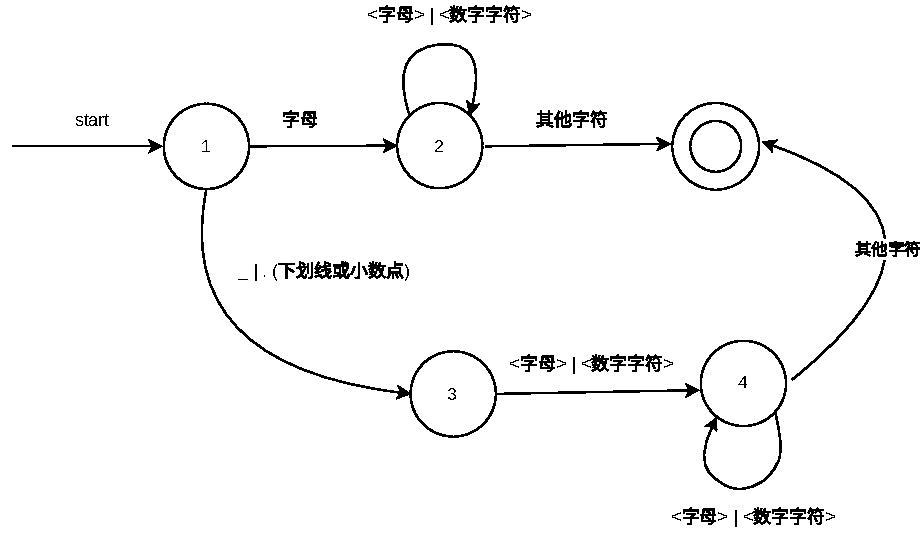
\includegraphics[width=0.8\linewidth]{2.1.drawio.pdf}
        \caption{标识符的状态图}
        \label{fig:2.1.drawio}
    \end{figure}

        \2 标识符:<字母>(<字母>|<数字字符>)*(ε|((\_|.)(<字母>|<数字字符>)+))

        描述:字母,或者以字母开头,后跟字母或数字的字符串,且字符间可以用一个下划线\_或一个小数点.相隔

        状态图见\cref{fig:2.1.drawio}。 变换后的正规文法:

        \begin{minted}{text}
    S→<字母>A
    A→<字母>A | <数字字符>A |ε| _B | .B
    B→<字母>B | <数字字符>B | <字母> | <数字字符>   
        \end{minted}

        \2 十进制数:((1|2|3|4|5|6|7|8|9) (0|1|2|3|4|5|6|7|8|9)*|0) (ε|(. (0|1|2|3|4|5 |6|7|8|9) (0|1|2|3|4|5|6|7|8|9)* ))

        \begin{figure}[htp]
            \centering
            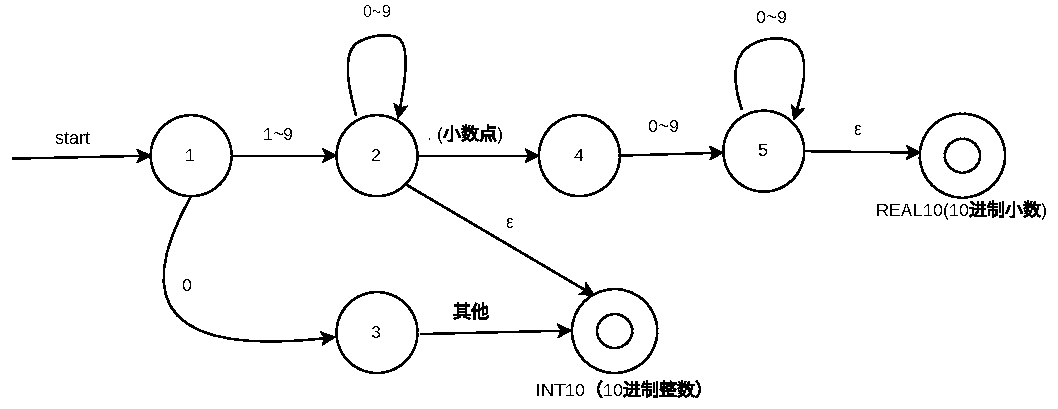
\includegraphics[width=0.8\linewidth]{2.2.drawio.pdf}
            \caption{十进制数的状态图}
            \label{fig:2.2.drawio}
        \end{figure}

        描述:整数部分为0-9,或者以不为0开头的由0-9组成的字符串,小数部分为0-9组成的字符串(整体的10进制字符串既可以是整数,也可以是小数)
        
        状态图见\cref{fig:2.2.drawio}。变换后的正规文法:

        \begin{minted}{text}
    S→ 1A | 2A | 3A | 4A | 5A | 6A | 7A | 8A | 9A| 0B
    A→ 0A | 1A | 2A | 3A | 4A | 5A | 6A | 7A | 8A | 9A| .C |ε
    B→ .C | ε
    C→ 0D | 1D | 2D | 3D | 4D | 5D | 6D | 7D | 8D | 9D
    D→ 0D | 1D | 2D | 3D | 4D | 5D | 6D | 7D | 8D | 9D | ε            
        \end{minted}

        \2 八进制数 0 (0|1|2|3|4|5|6|7)+ (ε|(.(0|1|2|3|4|5|6|7)(0|1|2|3|4|5|6|7)+))

        \begin{figure}[htp]
            \centering
            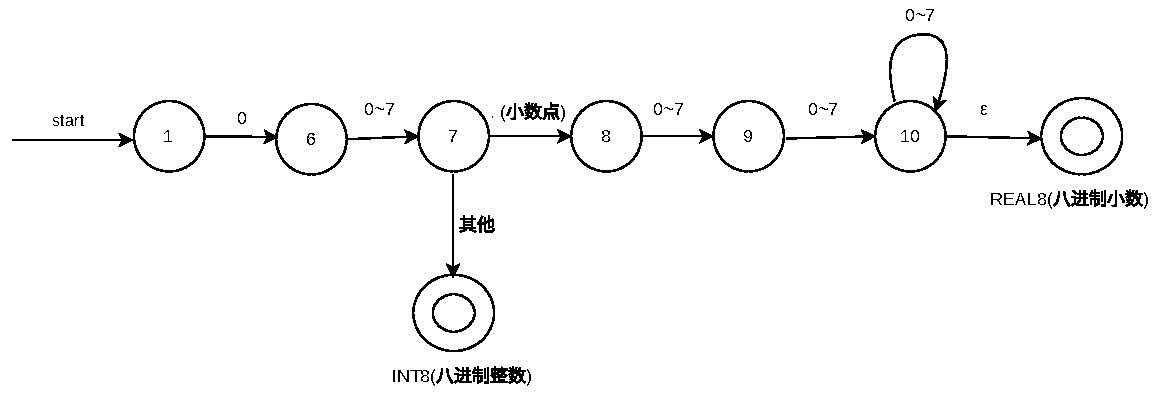
\includegraphics[width=0.8\linewidth]{2.3.drawio.pdf}
            \caption{八进制数的状态图}
            \label{fig:2.3.drawio}
        \end{figure}

        描述:以0开头由0-7组成的8进制字符串(既可以是整数,也可以是两位及以上小数)

状态图见\cref{fig:2.3.drawio}。变换后的正规文法:
\begin{minted}{text}
S→ 0A
A→ 0B | 1B | 2B | 3B | 4B | 5B | 6B | 7B
B→ 0B | 1B | 2B | 3B | 4B | 5B | 6B | 7B |ε| .C
C→ 0D | 1D | 2D | 3D | 4D | 5D | 6D | 7D
D→ 0E | 1E | 2E | 3E | 4E | 5E | 6E | 7E
E→ 0E | 1E | 2E | 3E | 4E | 5E | 6E | 7E |ε  
\end{minted}

\2 十六进制数  0x(0|1|2|3|4|5|6|7|8|9|a|b|c|d|e|f) (0|1|2|3|4|5|6|7|8|9|a|b|c\allowbreak |d|e|f)* (ε|(. (0|1|2|3|4|5|6|7|8|9|a|b|c|d|e|f)(0|1|2|3|4|5|6|7|8|9|a|\allowbreak b|c|d|e|f)+))

\begin{figure}[htp]
    \centering
    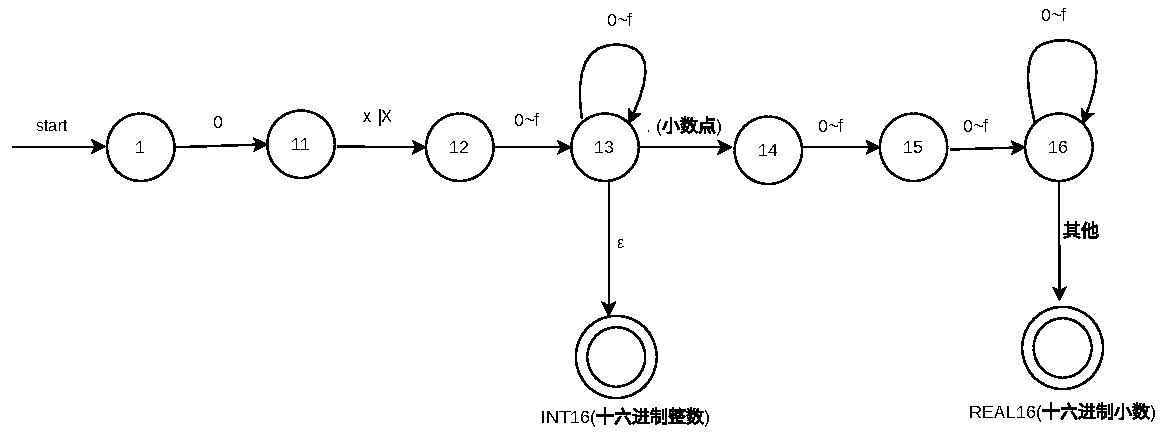
\includegraphics[width=0.8\linewidth]{2.4.drawio.pdf}
    \caption{十六进制数的状态图}
    \label{fig:2.4.drawio}
\end{figure}

描述:以0x开头由0-9,a-f组成的16进制整数或两位及以上小数

状态图见 \cref{fig:2.4.drawio} 变换后的正规文法:
\begin{minted}[breaklines]{text}
S→ 0xA | 0XA
A→ 0B | 1B | 2B | 3B | 4B | 5B | 6B | 7B | 8B | 9B | aB | bB | cB | dB | eB | fB
B→ 0B | 1B | 2B | 3B | 4B | 5B | 6B | 7B | 8B | 9B | aB | bB | cB | dB | eB | fB |ε| .C 
C→ 0D | 1D | 2D | 3D | 4D | 5D | 6D | 7D | 8D | 9D | aD | bD | cD | dD | eD | fD  
D→ 0E | 1E | 2E | 3E | 4E | 5E | 6E | 7E | 8E | 9E | aE | bE | cE | dE | eE | fE   
E→ 0E | 1E | 2E | 3E | 4E | 5E | 6E | 7E | 8E | 9E | aE | bE | cE | dE | eE | fE | ε
\end{minted}

\2 运算符和分隔符	+ | - | * | / | > | < | = | ( | ) | ;


\begin{figure}[htp]
    \centering
    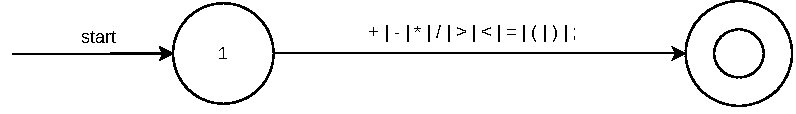
\includegraphics[width=0.8\linewidth]{2.6.drawio.pdf}
    \caption{运算符和分隔符的状态图}
    \label{fig:2.6.drawio}
\end{figure}

状态图见\cref{fig:2.6.drawio}。变换后的正规文法:

\begin{minted}{text}
S→ + | - | * | / | > | < | = | ( | ) | ;
\end{minted}

\2 关键字			if | then | else | while | do  

\begin{figure}[htp]
    \centering
    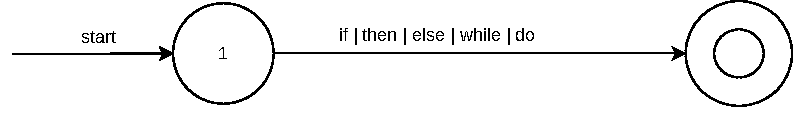
\includegraphics[width=0.8\linewidth]{2.7.drawio.pdf}
    \caption{关键字}
    \label{fig:2.7.drawio}
\end{figure}

状态图见\cref{fig:2.7.drawio}。变换后的正规文法:

\begin{minted}{text}
S→ if | then | else | while | do
\end{minted}

\begin{figure}[htp]
    \centering
    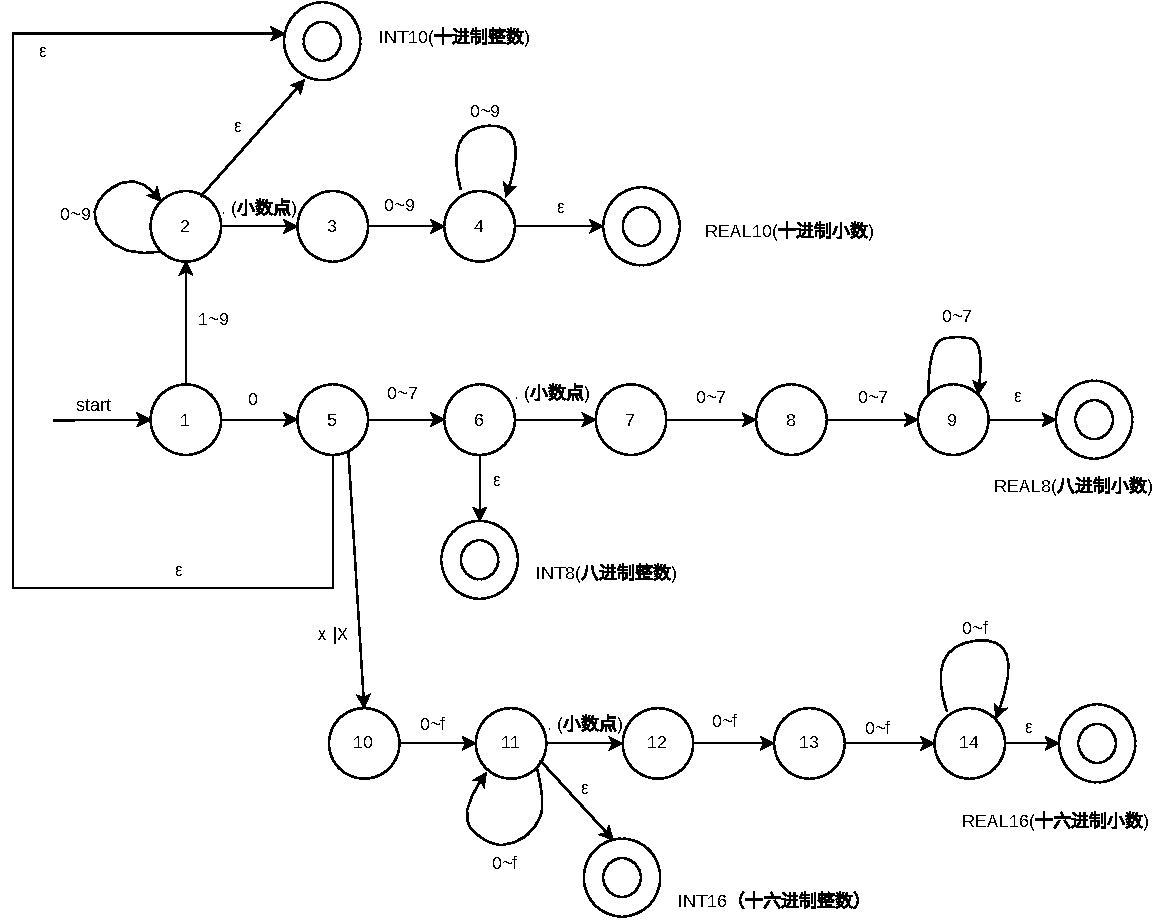
\includegraphics[width=0.8\linewidth]{2.5.drawio.pdf}
    \caption{整数的状态图}
\end{figure}
    \1 词法分析程序的数据结构与算法
\begin{minted}[breaklines]{c}
enum TYPE     //宏定义类别码
{
NONE,IDN,IF,THEN,ELSE,WHILE,DO,INT10,REAL10,INT8,REAL8,
INT16,REAL16,ADD,SUB,MUL,DIV,EQ,GT,LT,LP,RP,SEMI,ASG, WRONG=-1
};

char FILTER[4]={' ','\t','\r','\n'};//过滤符
bool IsFilter(char ch); //判断是否为过滤符
string KEYWORD[5] = {"if", "then", "else", "while", "do"};//关键字
int IsKeyword(string str);   //判断是否为关键字
bool IsLetter(char ch);   //判断是否为字母
bool IsDigit(char ch);    //判断是否是数字
int scan(FILE * fpin);  //从源程序文件中读取源程序,根据状态图来判断读入的字符进入哪个状态,从而判断字符串的类别,将其变换成相应的符号序列并以文件的形式存放

\end{minted}
        
\end{outline}



\section{语法分析子系统与三地址代码生成}
\subsection{实验目的}
掌握计算机语言的语法分析程序设计与属性文法应用的实现方法。采用适当的方法(递归子程序法、LL分析法、LR分析法,使用Yacc等自动生成工具),设计实现一个能够进行语法分析并生成三地址代码的微型编译程序。
\subsection{实验内容}
\subsubsection{预处理}
本子系统采用递归下降子程序法进行语法分析。首先需要对给定的文法进行消除左递归和提取左因子,具体过程如下所示:
\paragraph{源文法}
\begin{minted}{text}
P → L | LP
L → S 
S → id = E | if C then S | if C then S1 else S2 | while C do S | { P }
C → E > E | E < E | E = E
E → E + T | E - T | T
T → T * F | T / F | F
F → (E) | id | int8 | int10 | int16    
\end{minted}
\paragraph{消除左递归}
\begin{minted}{text}
P → LU
U → P | ε
L → S 
S → id = E | if C then S | if C then S1 else S2 | while C do S | { P }
C → E > E | E < E | E = E
E → TE’
E’ → +TE’
E’ → -TE’
E’ → ε
T → FT’
T’ → *FT’
T’ → /FT’
T’ → ε
F → (E) | id | int8 | int10 | int16    
\end{minted}
\paragraph{提取左因子}
\begin{minted}{text}
P → LU
U → P | ε
L → S 
S → id = E | if C then S | if C then S1 else S2 | while C do S | { P }
C → EC’
C’ → > E | < E | = E
E → TE’
E’ → +TE’ | -TE’ | ε
T → FT’
T’ → *FT’ | /FT’ | ε
F → (E) | id | int8 | int10 | int16    
\end{minted}
\subsection{系统结构说明}

语法分析子系统采用了递归子程序法。具体实现了proc\_P(), proc\_L(), proc\_S(), proc\_C(), proc\_E(), proc\_T(), proc\_F(),这7个子函数。
从P开始按照P,L,S,C,E,T,F的顺序深入,每一个子程序都会根据当前的 lookhead 值来确定当前读到的内容是否符合自己的产生式。若是就会根据对应的产生式去调用其他的子程序,并从中获取其 code 和 place 来根据语义规则生成自己的 code。并把自己的 code 返回上级。最后逐层返回上一级函数,直到返回到 P,P 会生成最终的三地址代码,并将其输出。
\subsubsection{数据结构说明}
\begin{outline}[enumerate]
    \1 \mintinline{c}{int Lookhead}:储存当前 lookahead 的状态。
        状态包括:NONE, IDN, IF, THEN, ELSE, WHILE, DO, INT10, REAL10, INT8,REAL8, INT16, REAL16, ADD, SUB, MUL, DIV, EQ, GT, LT, LP, RP, SEMI, ASG,WRONG
    \1 \mintinline{cpp}{String token}:储存当前 token 的值。
    \1 起始符 P, 非终结符 L 的结构体:
\begin{minted}{c}
struct P_Attr{
    string code; //存放P的代码
};
struct L_Attr{
    string code; //存放L的代码
};
\end{minted}
    \1 非终结符 S 的结构体:
\begin{minted}{c}
struct S_Attr{
    string code; //存放S的代码
    int  begin; //存放S的入口地址
    int  next; //存放S的出口地址
};
\end{minted}
    \1 非终结符 C 的结构体
\begin{minted}{c}
struct C_Attr{
    string code; //存放C的代码
    int  afalse; //存放C判断为假时的跳转标号
    int  atrue; //存放C判断为真时的跳转标号
};
\end{minted}
    \1 非终结符 F,T,E 的结构体:
\begin{minted}{c}
struct F_Attr{
    string code; //存放F的代码
    string place; //存放F的IDN值或int/real数值
};
struct T_Attr{
    string code; //存放T的代码
    string place; //存放T的IDN值或int/real数值
};
struct E_Attr{
    string code; //存放E的代码
    string place; //存放E的IDN值或int/real数值
};
\end{minted}
\end{outline}
\subsubsection{子函数说明}
\paragraph{Proc\_P()}
如\cref{fig:p} 和 \cref{fig:proc-p} 所示,分别是P的化简后的语法图和函数\texttt{P()}的流程图。函数P在执行过程中首先调用函数L()。在执行完函数L()之后,将结构体L的code值赋值给结构体P。然后会对当前的lookhead值进行判断。若lookhead不为空,说明;后面还有下一个表达式,需要传入结构体P1,递归调用函数P(P1)。若lookhead为空,说明语法分析已经完成,函数P结束。

\begin{figure}[htp]
    \centering
    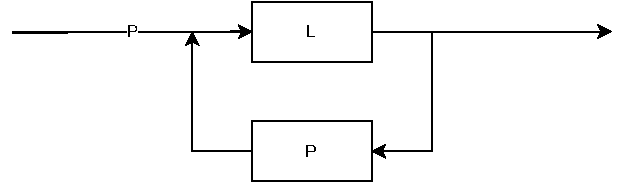
\includegraphics[width = .4\linewidth]{p.drawio.pdf}
    \caption{P的语法图}
    \label{fig:p}
\end{figure}

\begin{figure}[htp]
    \centering
    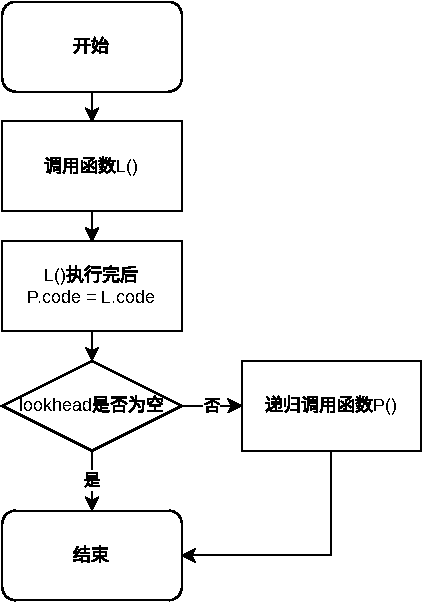
\includegraphics[width = .4\linewidth]{001P.drawio.png.pdf}
    \caption{函数P的流程图}
    \label{fig:proc-p}
\end{figure}
\paragraph{Proc\_S()}

\begin{figure}[htp]
    \centering
    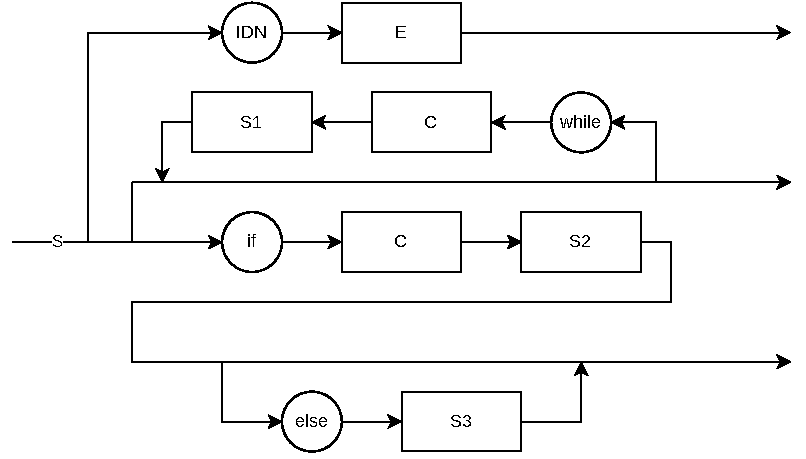
\includegraphics[width = .8\linewidth]{s.drawio.pdf}
    \caption{S的语法图}
    \label{fig:s}
\end{figure}

\begin{figure}[htp]
    \centering
    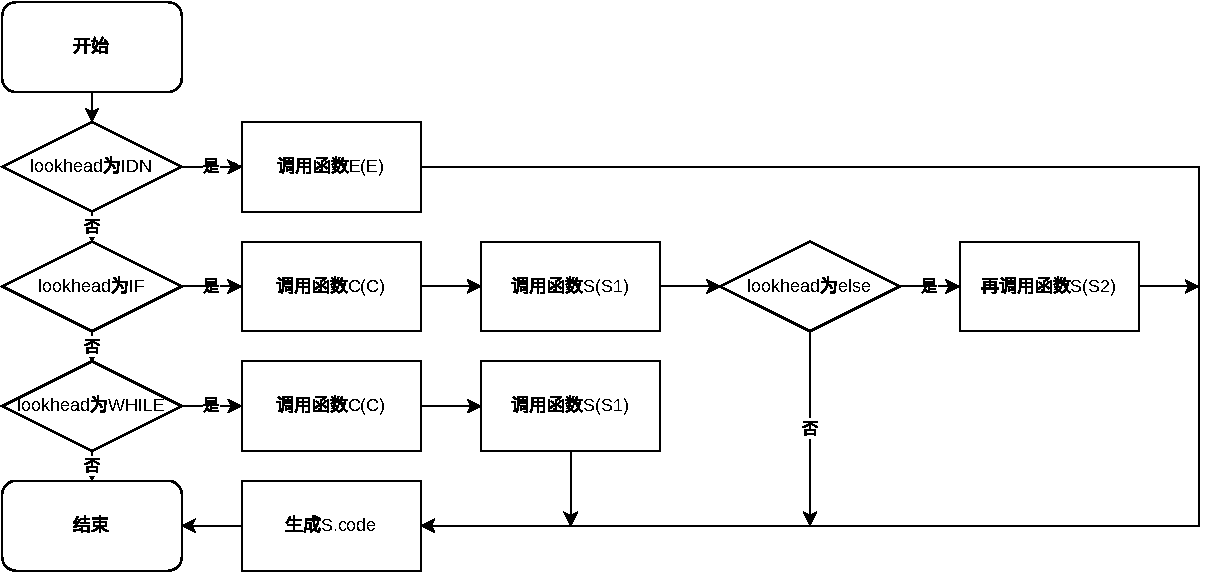
\includegraphics[width = .8\linewidth]{001S.drawio.png.pdf}
    \caption{函数S的流程图}
    \label{fig:proc-s}
\end{figure}

如\cref{fig:s} 和 \cref{fig:proc-s} 所示,分别是S的化简后的语法图和函数S()的流程图。函数S在执行过程中首先会判断lookhead的值。

若lookhead的值为IDN,说明当前处理的生成式是S->id=E。则传入结构体E,调用函数E(E),在函数E(E)执行完成后,根据语义规则:"S.code = E.code || gen(id.place’:=’E.place)",生成S.code= E.code + " \textbackslash{}n \textbackslash{}t" + IDN的值 + "=" + E.place。

若lookhead的值为IF,说明当前处理的生成式是S-> if C then S1或S-> if C then S1 else S2。则传入结构体C,调用函数C(C),在函数C(C)执行完成后,再传入结构体S1,递归调用函数S(S1)。然后再判断当前lookhead的值是否为else,若不为else,则根据语义规则"S.code = C.code || gen(C.true’:’) || S1.code"生成S.code= " \textbackslash{}n \textbackslash{}t" + C.code + " \textbackslash{}nL" + C.atrue + ": \textbackslash{}t" + S1.code; 若为else,则继续递归调用函数S(S2),最后根据语义规则"S.code = C.code || gen(C.true’:’) || S1.code|| gen(‘goto’S.next)|| gen(C.false’:’)|| S2.code;"生成S.code= " \textbackslash{}n \textbackslash{}t" + C.code + " \textbackslash{}nL" + C.atrue + ": \textbackslash{}t" + S1.code + " \textbackslash{}nL" + C.afalse + ": \textbackslash{}t" + S2.code。{\setlength{\emergencystretch}{.3em}\par}

若lookhead的值为WHILE,说明当前处理的生成式是S-> while C do S。则传入结构体C,调用函数C(C),在函数C(C)执行完成后,再传入结构体S1,递归调用函数S(S1)。最后根据语义规则"S.code = gen(S.begin’:’) || C.code || gen(C.true’:’) || S1.code || gen(‘goto’S.begin);"生成S.code= S->code = " \textbackslash{}nL" + S->begin + ": \textbackslash{}n \textbackslash{}t" + C.code + " \textbackslash{}nL" + C.atrue + ": \textbackslash{}t" + S1.code + " \textbackslash{}n \textbackslash{}tgoto L" + S->begin{\setlength{\emergencystretch}{.14em}\par}

\paragraph{PROC\_C()}
\begin{figure}
    \centering
    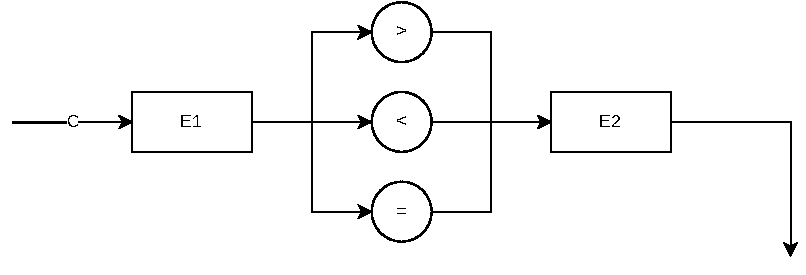
\includegraphics[width = .8\linewidth]{c.drawio.pdf}
    \caption{C的语法图}
    \label{fig:c}
\end{figure}
\begin{figure}
    \centering
    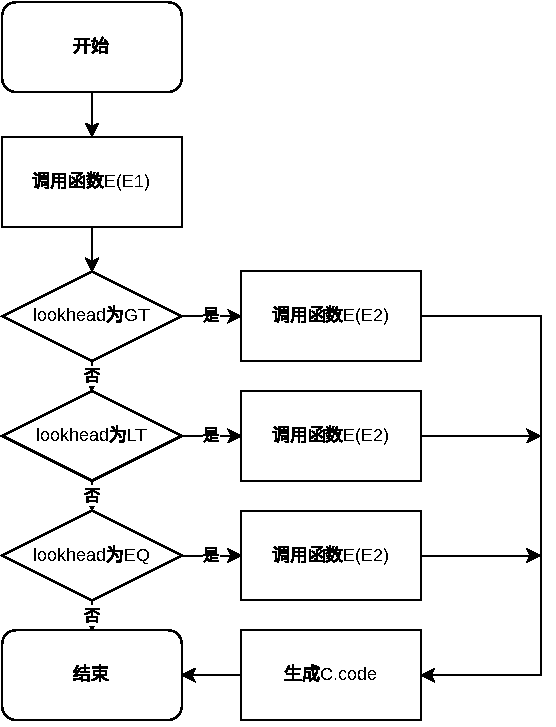
\includegraphics[width = .4\linewidth]{001C.drawio.png.pdf}
    \caption{函数C的流程图}
    \label{fig:proc-c}
\end{figure}

如\cref{fig:c} 和 \cref{fig:proc-c} 所示,分别是C的化简后的语法图和函数C()的流程图。函数C在执行过程中首先会传入结构体E1,调用函数E(E1)。在函数E(E1)执行完后,判断lookhead的值。

若lookhead的值为GT,说明当前处理的生成式是C-> E1>E2。则传入结构体E2,调用函数E(E2),在函数E(E)执行完成后,根据语义规则:“C.code = E1.code || E2.code ||gen(‘if’E1.place’>’E2.place’goto’C.true) ||gen(‘goto’C.false)”,生成C.code= E1.code + E2.code + "\textbackslash{}n\textbackslash{}t if " + E1.place + ">" + E2.place + " goto L" + C->atrue + "\textbackslash{}n\textbackslash{}t goto L" + C->afalse。

若lookhead的值为LT,说明当前处理的生成式是C-> E1<E2。则传入结构体E2,调用函数E(E2),在函数E(E)执行完成后,根据语义规则:“C.code = E1.code || E2.code ||gen(‘if’E1.place’<’E2.place’goto’C.true) ||gen(‘goto’C.false)”,生成C.code= E1.code + E2.code + "\textbackslash{}n\textbackslash{}t if " + E1.place + "<" + E2.place + " goto L" + C->atrue + "\textbackslash{}n\textbackslash{}t goto L" + C->afalse。

若lookhead的值为EQ,说明当前处理的生成式是C-> E1=E2。则传入结构体E2,调用函数E(E2),在函数E(E)执行完成后,根据语义规则:“C.code = E1.code || E2.code ||gen(‘if’E1.place’=’E2.place’goto’C.true) ||gen(‘goto’C.false)”,生成C.code= E1.code + E2.code + "\textbackslash{}n\textbackslash{}t if " + E1.place + "=" + E2.place + " goto L" + C->atrue + "\textbackslash{}n\textbackslash{}t goto L" + C->afalse。

\paragraph{PROC\_E()}
\begin{figure}
    \centering
    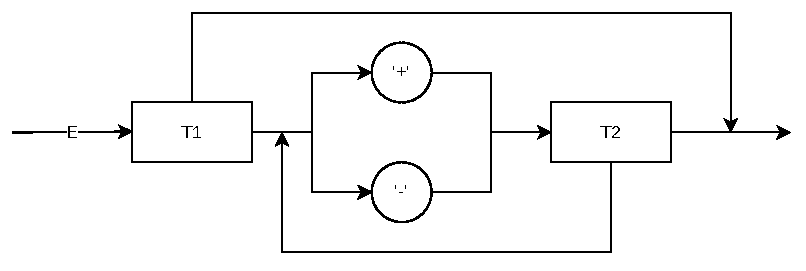
\includegraphics[width = .8\linewidth]{e.drawio.pdf}
    \caption{E的语法图}
    \label{fig:e}
\end{figure}
\begin{figure}
    \centering
    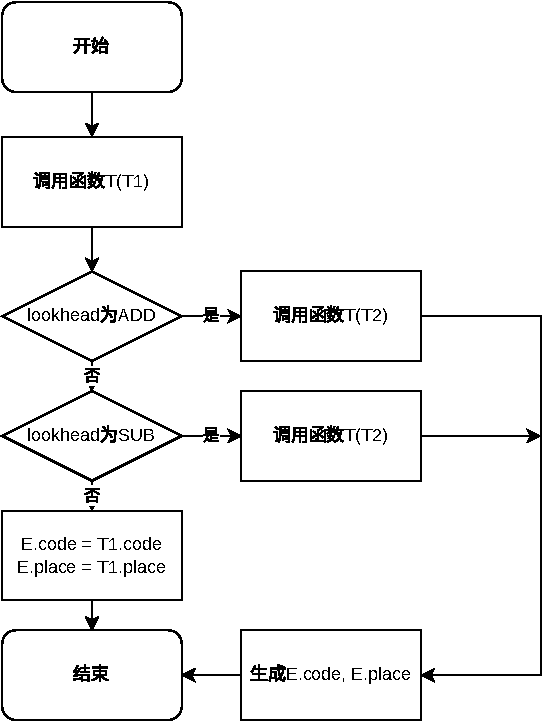
\includegraphics[width = .4\linewidth]{001E.drawio.png.pdf}
    \caption{函数E的流程图}
    \label{fig:proc-e}
\end{figure}
如\cref{fig:e} 和 \cref{fig:proc-e} 所示,分别是E的化简后的语法图和函数E()的流程图。函数E在执行过程中首先会传入结构体T1,调用函数T(T1)。在函数T(T1)执行完后,判断lookhead的值。

若lookhead的值为ADD,说明当前处理的生成式是E->T1 + T2。则传入结构体T2,调用函数T(T2),在函数T(T2)执行完成后,根据语义规则:“E.code = T1.code||T2.code||gen(E.place’:=’T1.place’+’T2.place)”,生成E.code= T1.code+T2.code + "\textbackslash{}n" + "\textbackslash{}t" + E->place + "=" + T1.place + " + " + T2.place。

若lookhead的值为SUB,说明当前处理的生成式是E->T1 - T2。则传入结构体T2,调用函数T(T2),在函数T(T2)执行完成后,根据语义规则:“E.code = T1.code||T2.code||gen(E.place’:=’T1.place’-’T2.place)”,生成E.code= T1.code + T2.code + "\textbackslash{}n" + "\textbackslash{}t" + E->place + "=" + T1.place + "-" + T2.place。

若lookhead不是上述;两个值中的任何一个,说明当前产生式不是E的产生式处理的,此时将T1的code和place赋值给E,然后结束函数。

\paragraph{PROC\_T()}
\begin{figure}
    \centering
    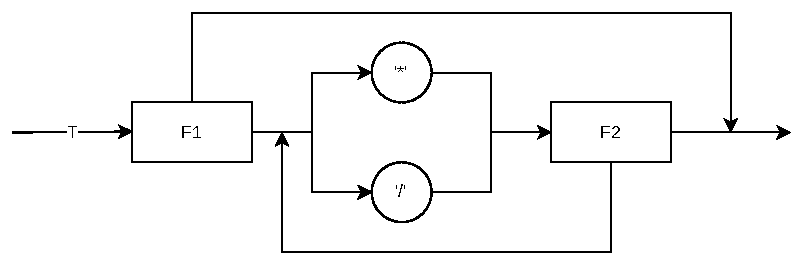
\includegraphics[width = .8\linewidth]{t.drawio.pdf}
    \caption{T的语法图}
    \label{fig:t}
\end{figure}
\begin{figure}
    \centering
    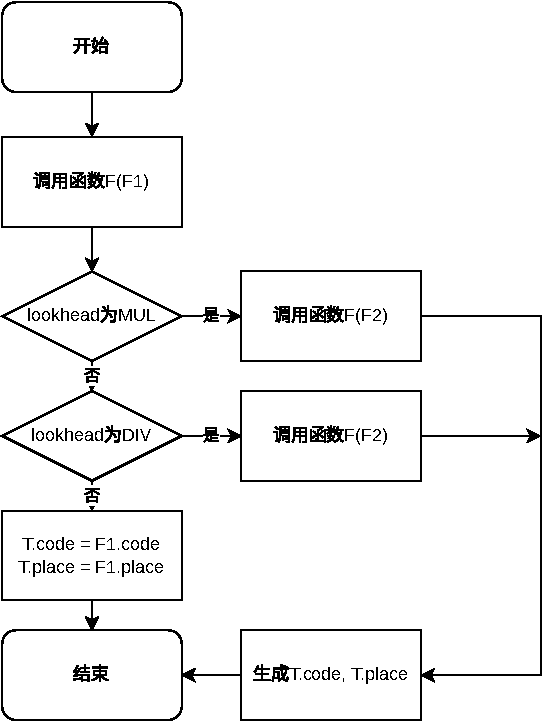
\includegraphics[width = .4\linewidth]{001T.drawio.png.pdf}
    \caption{函数T的流程图}
    \label{fig:proc-t}
\end{figure}
如\cref{fig:t} 和 \cref{fig:proc-t} 所示,分别是T的化简后的语法图和函数E()的流程图。函数T在执行过程中首先会传入结构体F1,调用函数F(F1)。在函数F(F1)执行完后,判断lookhead的值。
若lookhead的值为MUL,说明当前处理的生成式是T->F1 * F2。则传入结构体F2,调用函数F(F2),在函数F(F2)执行完成后,根据语义规则:“T.code = F1.code || F2.code ||gen(T.place’:=’F1.place’*’F2.place)”,生成F.code= F1.code + F2.code + "\textbackslash{}n" + "\textbackslash{}t" + T->place + "=" + F1.place + "*" + F2.place。

若lookhead的值为DIV,说明当前处理的生成式是T->F1 / F2。则传入结构体F2,调用函数F(F2),在函数F(F2)执行完成后,根据语义规则:“T.code = F1.code || F2.code ||gen(T.place’:=’F1.place’/’F2.place)”,生成F.code= F1.code + F2.code + "\textbackslash{}n" + "\textbackslash{}t" + T->place + "=" + F1.place + "/" + F2.place。

若lookhead不是上述;两个值中的任何一个,说明当前产生式不是T的产生式处理的,此时将F1的code和place赋值给T,然后结束函数。

\paragraph{PROC\_F()}
\begin{figure}
    \centering
    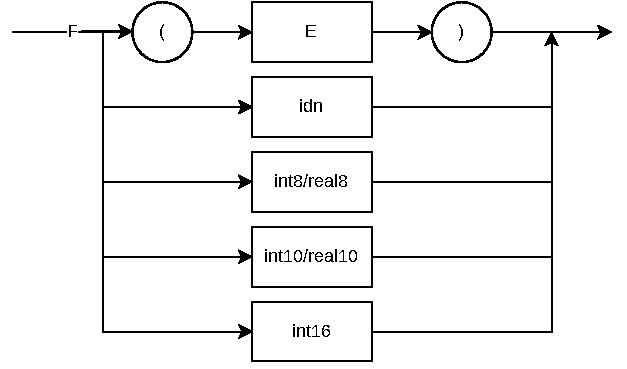
\includegraphics[width = .8\linewidth]{f.drawio.pdf}
    \caption{F的语法图}
    \label{fig:f}
\end{figure}
\begin{figure}
    \centering
    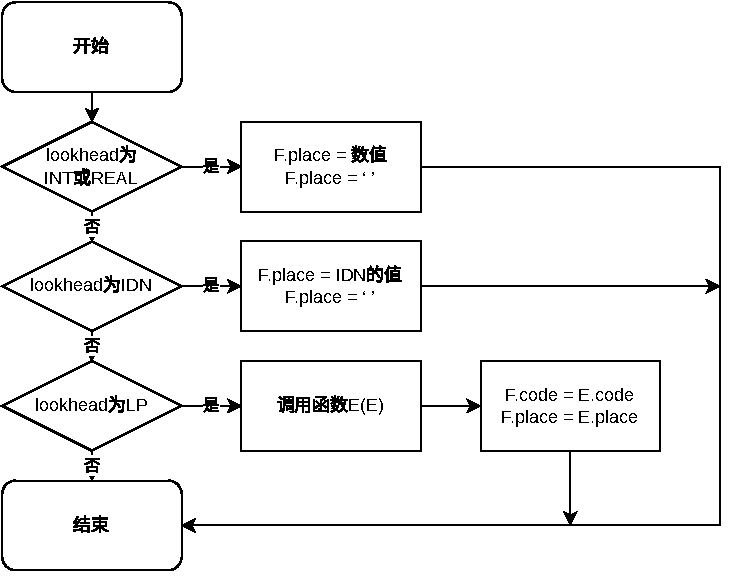
\includegraphics[width = .8\linewidth]{001F.drawio.png.pdf}
    \caption{函数F的流程图}
    \label{fig:proc-f}
\end{figure}
如\cref{fig:f} 和 \cref{fig:proc-f} 所示,分别是F的化简后的语法图和函数F()的流程图。函数F首先会判断lookhead的值。

若lookhead的值为INT8,INT10,INT16,REAL8,REAL10或REAL16,说明当前处理的生成式是F-> INT8|INT10|INT16|REAL8|REAL10|REAL16。此时,将读取到的数值转化成10进制数赋值给F.place,F.code = ‘ ’。

若lookhead的值为IDN,说明当前处理的生成式是F-> id。此时,将读取到的标识符id的值赋值给F.place,F.code = ‘ ’

若lookhead的值为LP;说明当前处理的生成式是F-> (E)。传入结构体E,调用函数E(E),在函数E(E)执行完成后,将E的code和place赋值给F,然后结束函数。

\subsection{实验结果}
\subsubsection{测试1}
输入:
\begin{minted}{text}
while (a3+15)>0xa do if x2 = 7.233 then while y<z do y = x * y / z; c=b*c+d;
\end{minted}

输出:

\begin{minted}{tex}
L1:
    t1=a3+15.000000
    if t1>10.000000 goto L2
    goto L0
L2:
    if x2=7.233000 goto L3
    goto L1
L3:
L4:
    if y<z goto L5
    goto L1
L5:
    t2=x*y
    t3=t2/z
    y=t3
    goto L4
    goto L1
L0:
    t4=b*c
    t5=t4+d
    c=t5
\end{minted}

如上所示,输入为实验指导书中所提供的。观察可知,三地址码生成正确。

\subsubsection{测试2}
输入:

\begin{minted}{text}
while (a3+15)>0xa 
    do if x2 = 07 
      then while y<z 
        do y = x * y / z; 
  c=b*c+d;
\end{minted}

输出
\begin{minted}{text}
L1:
    t1=a3+15.000000
    if t1>10.000000 goto L2
    goto L0
L2:
    if x2=7.000000 goto L3
    goto L1
L3:
L4:
    if y<z goto L5
    goto L1
L5:
    t2=x*y
    t3=t2/z
    y=t3
    goto L4
    goto L1
L0:
    t4=b*c
    t5=t4+d
    c=t5
\end{minted}

如上所示,输入同测试1为实验指导书中所提供的,但是在其中加入了换行符。观察可知,三地址码生成正确。

\subsubsection{测试3}
输入:
\begin{minted}[breaklines]{text}
while (a3+15)>0xa do if x2 = 7.233 then while y<z do while a<1 do y = x * y / z; c=b*c+d;
\end{minted}

输出:
\begin{minted}{text}
L1:
    t1=a3+15.000000
    if t1>10.000000 goto L2
    goto L0
L2:
    if x2=7.233000 goto L3
    goto L1
L3:
L4:
    if y<z goto L5
    goto L1
L5:
L6:
    if a<1.000000 goto L7
    goto L4
L7:
    t2=x*y
    t3=t2/z
    y=t3
    goto L6
    goto L4
    goto L1
L0:
    t4=b*c
    t5=t4+d
    c=t5
\end{minted}

如上所示,输入在实验指导书中所提供的代码基础上增加了一重循环。观察可知,三地址码生成正确。

\subsubsection{测试4}
输入:
\begin{minted}{text}
if a<1 then a=a+1 else a=a-1
\end{minted}

输出:
\begin{minted}{text}
if a<1.000000 goto L1
    goto L0
L1:
    t2=a+1.000000
    a=t2
L0:
    t3=a-1.000000
    a=t3
\end{minted}
如上所示,输入为“if a<1 then a=a+1 else a=a-1”。此输入可以用来测试E->T1+T2;E->T1-T2;C->E1<E2和S-> if C then S1 else S2。观察可知,三地址码生成正确。

\subsubsection{测试5}
输入:
\begin{minted}{text}
if a>1 then a=a*2 else a=a/4;
\end{minted}

输出:
\begin{minted}{text}
if a>1.000000 goto L1
    goto L0
L1:
    t2=a*2.000000
    a=t2
L0:
    t3=a/4.000000
    a=t3
\end{minted}

如上所示,输入为“if a>1 then a=a*2 else a=a/4;”。此输入可以用来测试T->F1*F2;T->F1/F2;C->E1>E2和S-> if C then S1 else S2。观察可知,三地址码生成正确。

\subsubsection{测试6}
输入:
\begin{minted}{text}
if a=1 then a=a+3
\end{minted}

输出:
\begin{minted}{text}
if a=1.000000 goto L1
    goto L0
L1:
    t1=a+3.000000
    a=t1
L0:
\end{minted}

如上所示,输入为“if a=1 then a=a+3”。此输入可以用来测试F->(E);F->IDN;F->INT10和S-> if C then S1。观察可知,三地址码生成正确。

\subsubsection{测试7}
输入:
\begin{minted}{text}
while a>2 do a=a-1;
\end{minted}

输出:
\begin{minted}{text}
L1:

    if a>2.000000 goto L2
    goto L0
L2:
    t1=a-1.000000
    a=t1
    goto L1
L0:
\end{minted}

如上所示,输入为“while a>2 do a=a-1;”。此输入可以用来测试S-> while C do S1。观察可知,三地址码生成正确。


\chapter{LR分析表自动构建系统}
\section{实验内容}
LR分析法是一种能根据当前分析栈中状态和向右顺序查看输入串符号就可以唯一确定分析器的动作是移进还是归约,以及用哪个产生式归约的自底向上语法分析算法。对于LR(0),给定文法,在分析过程中需要LR(0)的分析表对下一步的操作进行分析。

LR分析表具体包括ACTION表和GOTO表,ACTION表告诉分析器栈顶状态为i时,对于下一个输入符号应如何操作;GOTO表表示了当前栈顶状态为i时,遇到文法应该转向哪个状态。

LR分析表的生成过程大致流程为:先从S’->S开始,求闭包,然后产生下一个状态的文法,再求闭包,以此类推。直到没有更多的状态产生。在编写的程序中,会将每个状态编号,并保存每个状态的父子状态,方便输出分析表。

\section{实验结果}

\subsection{数据结构}
\subsubsection{Sentence类}
Sentence类是文法的数据结构,存储文法的内容、文法点的位置。
\begin{minted}{cpp}
class Sentence{
    public:
        string str;
        int dot;

        Sentence(string str){
            this->str = str;
            this->dot = 0;
        }
        void addDot(void){          //添加"."
            this->str.insert(3,".");
            this->dot = 3;
        }
        void moveDot(void){         //后移一位"."
            this->str[this->dot] = this->str[this->dot+1];
            this->str[this->dot+1] = '.';
            this->dot += 1;
        }
        void print(){
            cout << str << endl;
        }
};
\end{minted}
\subsubsection{DFA类}
DFA存储状态,包括状态包含的文法、状态编号等。
\begin{minted}{cpp}
class DFA{
    public:
        vector<Sentence> sentences;
        int num;//序号
        int fatherNum;
        vector<int> sonNum;
        DFA(Sentence sentences){
            this->sentences.push_back(sentences);
            this->num = Snum;
            Snum++;
            this->fatherNum = -1;
        }
        void print(){
                cout << num<<endl;
            for(auto i:sentences){
                i.print();
            }
            cout << "father: " << this->fatherNum << endl;
            cout << "son: ";
            for(auto i:sonNum)
                cout << i << " ";
            cout << endl;
        }
};
\end{minted}
\subsection{主要函数功能}
\subsubsection{Init函数}
Init函数生成一个新的文法 S' 作为第一个状态的文法,并求其闭包。
\begin{minted}{cpp}
void Init(){
    int i;
    ifstream in("test.txt");        //输入的文档名
    if(!in.is_open())               //判断一下是否正常打开
        cout << "Error";            //失败返回输出
    for (i = 1;;i++){               //将每一句文法按照Sentence存入input中
        string str;
        in >> str;
        if(str=="#")                //遇到#表明结束了
            break;
        Sentence s = Sentence(str);
        input.push_back(s);
    }
    string str = "Z->";             //创建新的文法Z->S
    str.push_back(input[0].str[0]);
    Sentence s = Sentence(str);
    s.addDot();                     //新文法Z->.S
    DFA dfa = DFA(s);               //把这个新文法放入第一个状态中。
    LR.push_back(dfa);              //存储状态
}
\end{minted}
\subsubsection{addSentence函数}
addSentence函数对传入的状态求闭包。
\begin{minted}{cpp}
void addSentence(DFA &dfa){             //给状态添加闭包
    //获得点后面的非终结符
    char c = dfa.sentences[0].str[dfa.sentences[0].dot + 1];
    for(auto s:getSetence(input,c)){    //在输入的文法中找终结符相同的
        s.addDot();                     //给文法加上点
        dfa.sentences.push_back(s);     //把修改后的文法添加到该状态中
    }
}
\end{minted}
\subsubsection{findSon函数}
findSon函数遍历生成的状态,找到每个状态的父子状态。
\begin{minted}[breaklines]{cpp}
void findSon(){
    for (int i = 0; i < LR.size();i++){
        // 删除重复的状态
        // compare函数把传入的状态跟所有状态的第一个文法作比较,如果有相同的返回true
        if(compare(LR[i])){
            LR.erase(LR.begin()+i);
            i--;
            continue;
        }
        // 添加语句
        addSentence(LR[i]);// 给状态添加闭包
        //扩散
        for(auto s:LR[i].sentences){    // 对于状态中的每个句子
            if(s.dot+1==s.str.length()) // 如果点的位置已经到结尾了,不再添加新状态
                continue;
            Sentence tempS = s;         // 点没到结尾,添加新状态
            tempS.moveDot();            // 将点的位置向后移一个
            LR.push_back(DFA(tempS));   // 创建新的状态,将移动后的文法添加到状态中
        }
    }
    for (int i = 0; i < LR.size();i++)
        LR[i].num = i;//重编号
    for (int i = 0; i < LR.size();i++){                 // 遍历生成的这些状态
        for(auto sentence:LR[i].sentences){             // 遍历状态的文法
            if(sentence.dot+1==sentence.str.length())   // 跳过结束的文法
                continue;
            Sentence tempS = sentence;
            // 找子状态,所以文法的点向后移动一个,在其他状态中找第一个文法与这个结果相同的状态。
            tempS.moveDot();
            // 爹不能是自己
            for (int t = 0; t < LR.size();t++){         // 遍历其他状态
                if(LR[t].sentences[0].str==tempS.str){  // 如果找到了
                    if(t!=i)//不是自己
                    LR[t].fatherNum = i;        // 将找到的子状态的父亲标为当前状态
                    LR[i].sonNum.push_back(t);  // 当前状态记录子状态的标号
                }
            }
         }
    }
}
\end{minted}

\subsection{实验结果}
输入文法:
\begin{minted}{text}
E->aA
E->bB
A->cA
A->d
B->cB
B->d
#
\end{minted}
输出的分析表:
\begin{minted}{text}
    ACTION           GOTO
     a    b    c    d    #    E    A    B
0:   S2   S3                  1
1:                       acc
2:             S5   S9             4
3:             S7   S11                 6
4:   r0   r0   r0   r0   r0
5:             S5   S9             8
6:   r2   r2   r2   r2   r2
7:             S7   S11                 10
8:   r4   r4   r4   r4   r4
9:   r5   r5   r5   r5   r5
10:  r6   r6   r6   r6   r6
11:  r7   r7   r7   r7   r7
\end{minted}

\chapter{面向LLVM IR的类C语言编译器}
本项目完成了一个面向LLVM IR\cite{lattnerLLVMCompilationFramework2004}的类C语言编译器,支持任意维数的数组、指针、结构体等特性,可由LLVM的编译器编译为各个平台的可执行程序,可链接C ABI的动态或静态库。下面,为本项目做一个简单的介绍。
\section{\cb 语言设计}
本项目实现了一个简易的C语言。正如微软的、比C语言多一些功能和特性的,『升C(\cs)』语言,我们的语言比C语言少一些特性,因此称为『降C(\cb)』。

语言的设计部分参考了《自制编译器\cite{qingmufenglangZiZhiBianYiQi}》书籍中的\cb 语言,并为了实验作出了部分调整。总体上来说,\cb 语言与C语言的区别如下:
\begin{outline}[enumerate]
    \1 类型定义中,后置声明(如\texttt{*, []}) 前移
\begin{minted}{c}
int a[5];    -->  int[5] a;
int *a, b;   -->  int* a; int b;
\end{minted}
        这样修改后,更符合现代语言(如Rust、Java)等的设计,更贴合直觉。
    \1 支持块注释的嵌套

        得益于优秀的词法分析设计,\cb 支持块注释的嵌套使用:
\begin{minted}{text}
/* 123
/* 233
*/
*/
\end{minted}
    \1 函数控制流结束时,如果没有写 return 语句,则会隐式返回对应类型的 0 值
        
        在传统 C 语言中,这是未定义行为,代码优化时往往会假设这一行为不会发生,会导致初学者对于类似行为的疑惑。在 \cb 语言中,我们定义此时会返回0值。
    \1 预处理器

        由于本课程的重点并不包括预处理器,因此并没有实现预处理器,本编译器脱离预处理器也可以单独运行。如果想要使用类似头文件的功能,\cb 语言也兼容使用C语言的预处理器(如\texttt{cpp}命令)。
    \1 浮点数

        由于工作量限制,\cb 语言的\emph{语法、语义解析与代码生成部分}不支持浮点数。
        \emph{词法分析}部分支持浮点数,符合实验指导书中『附加要求』。
    \1 \texttt{enum}

        作为整数常量的语法糖,C语言中的\texttt{enum}特性并没有得到广泛的使用。同样处于工作量角度考虑,\cb 不支持\texttt{enum}。
    \1 结构体的位域

        位域(bitfield)是一个很少被听说、使用的C语言特性。同样,由于其很少被使用且因为工作量限制,\cb 不支持位域。
    \1 \texttt{volatile, register}

        由于\cb 编译为LLVM IR,由LLVM完成优化;同时C语言标准中,\texttt{register}关键字也仅仅是『建议』编译器将变量放置在寄存器中,现代编译器常常会不理会这个『建议』。因此,\cb 不支持这两个关键字。
    \1 \texttt{const}、自引用类型(如结构体中包括指向自己的域)、\texttt{while}与\texttt{do-while}循环
        
        以上特性不影响语言的图灵完备性,均可通过其他方式达到(如使用\texttt{void*}指针和类型转换实现结构体中包括指向自己的域、使用\texttt{for}循环替代\texttt{while}循环),因此,出于工作量角度考虑,\cb 不支持以上特性。
    
    \1 内联汇编

        对于一门课程的实验来讲,内联汇编特性过于复杂。因此,\cb 不支持内联汇编。

        不支持内联汇编意味着\cb 无法直接发起系统调用。但是,\cb 支持各种各样的Calling Convension,在各个平台上均能动态或静态链接C语言标准库(如musl、glibc),因此可以通过C语言标准库提供的\texttt{printf/scanf}等函数提供输入输出支持。
\end{outline}
\subsection{程序示例}
本程序演示了\cb 语言的大部分特性。
\begin{minted}[breaklines]{c}
// 注:此处使用了C语言的代码高亮,因此使用部分C语言不支持的特性(如块注释嵌套)的代码高亮会显示错误。
/* /* 块注释的嵌套 */ */
int a = 0x1234;                                 // 全局变量定义
int b = 'a';
char c = 3 + 235;                               // 编译时常量定义
extern int printf(char*, ...);                  // 外部函数声明
char * str = "___Hello world from Cb lang!\n";  // 字符串字面量
struct test{                                    // 结构体定义
    int foo;
    char bar;
};
int add(int a, int[] b){                        // 接受任意长度数组、返回整数的函数定义
    return a + b[0];
}
struct test fooo(void){                         // 返回结构体的函数定义
    struct test ret;
    ret.foo = 2;
    ret.bar = 'c';
    return ret;
}
int main(int argc, char** argv){                // 类C语言的main函数,支持命令行参数
    auto ret = fooo();                          // auto关键字
    printf("%d %c\n", ret.foo, ret.bar);        // 调用外部函数
    int[5][2] array;                            // 多维数组
    int[5]* array_ptr = array;                  // 转为数组指针
    struct test ss;
    struct test* ss_pointer = &ss;              // 结构体指针
    ss.foo = 1234;                              // 结构体赋值
    printf(&str[3]);                            // 对指针使用下标访问运算符、对右值取地址
    printf(str + 3);                            // 指针的数学运算
    printf("This is %d %d\n", 2 + 1238796, a);  // 函数调用中的数学运算
    printf("Argc: %d\n", argc);                 // 命令行参数
    array[0][0] = 0x123;                        // 数组访问
    printf("array[0][0] = %d\n", array[0][0]);
    printf("array_ptr[0][0] = %d\n", array_ptr[0][0]);
    if(argc == 1) {                             // if语句
        printf("Then\n");
        return -1;                              // return语句
    } else {
        printf("Else\n");
    }
    printf("%d\n", ss.bar);
    int* pointer = &ss.bar;                     // 对结构体的域取地址
    *pointer = 0x1234;                          // 指针解引用
    printf("%d\n", ss.bar);
    ss_pointer->foo = 0;                        // 结构体指针使用->运算符
    printf("%d\n", ss.foo);
    printf("A + B = %d\n", add(2, array[0]));   // 将二维数组中的一维数组作为参数
    printf("argv: %s\n", argv[0]);
    1 && printf("not_reached");                 // 按位与运算符的短路
    0 && printf("good\n");
    0 || printf("not_reached");                 // 按位或运算符的短路
    1 || printf("good\n");
    (0,1) || printf("good\n");                  // 逗号表达式
    printf("1+2*3=%d\n", 1 + 2 * 3 * 3 / 3);
    if (!1) {
        printf("not reached");
    } else {
        printf("good\n");
    }
    int i = 0;
    for(i = 0; i < argc; ++ i){                 // for循环
        if (i == 3){
            printf("Break!");
            break;                              // break语句
        } else if(i == 2){
            printf("Contine!");
            continue;                           // continue语句
        }
        printf("for %d\n", i);
    }
}

\end{minted}

\section{工具选择}

% \runcompiler{../tests/error.cb}

\subsection{词法与语法生成器}
本编译器采用ANTLR\cite{parrANTLRPredicatedLLParser1995}(ANother Tool for Language Recognition)作为词法、语法解析器的生成器。ANTLR基于递归下降生成语法解析程序,支持ALL*(Adaptive LL(*))文法,比传统的LL(*)适用性更广。同时,相比yacc等基于LR的解析器生成器,基于递归下降这一点使得他生成的代码更可读。同时,ANTLR具有优秀的错误处理和恢复能力,可以处理词法和词法分析过程中出现的绝大部分错误。他还支持在语法解析的过程中内联动作, 这使得他可以在语法分析的同时完成语义分析。由以上原因,本编译器采用ANTLR作为词法和语法解析器的生成器。

\subsection{编程语言}
本编译器采用Rust语言编写。在编译器这个项目上,使用Rust语言具有以下优势:
\begin{outline}
    \1 Tagged Union 与 Pattern Matching

        Rust语言独有的 Tagged Union 非常适合在编写编译器过程中可能会用到的数据结构。如,以下代码是 \cb 编译器的类型节点的定义:
\begin{minted}[breaklines]{rust}
pub enum Type {
    Void,
    Integer {
        signed: bool,
        size: usize,
    },
    Array {
        size: usize,
        element_type: Arc<Type>,
    },
    Function {
        return_type: Arc<Type>,
        parameters: Vec<(String, Arc<Type>)>,
        variadic: bool,
    },
    Pointer {
        element_type: Arc<Type>,
    },
    Struct {
        name: String,
        fields: Vec<(String, Arc<Type>)>,
        location: Range<usize>,
    },
}
\end{minted}
        使用 Tagged Union 与 Pattern Matching 可以有效减少重复的代码量,并减少现代面向对象语言中虚表的开销。
    \1 编译时的生命周期检查

        Rust将引用的生命周期作为类型系统的一部分,使得其可以在编译时进行变量引用的声明周期检查。这使得Rust可以称为『内存安全的编程语言』,也就是说,只要不使用 \texttt{unsafe} 关键字,代码就不会出现未定义行为。

        在编写编译器的过程中,抽象语法树节点之间会互相引用,在这样一个具有大量对象的引用的场景下,如果使用C++等传统语言,若代码写错一点就可能造成程序段错误,难以排查。使用Rust则可以在编译时解决这类问题,加快项目开发的速度与时间。
\end{outline}

\subsection{中间表示语言}

本项目采用LLVM IR\cite{lattnerLLVMCompilationFramework2004}作为中间表示语言,并使用LLVM编译器输出最终的可执行文件。LLVM IR作为一种底层的中间表示语言,其形式更像是汇编。他抽象了各个目标平台不同的部分,提供了一个统一的接口,提供强大的优化能力,使得编写编译器的人可以专注于前端。现代的编程语言或编译器,如Rust、Clang等,均使用LLVM作为后端,在减少工作量的同时接入LLVM生态,支持多种目标平台。

LLVM 虚拟机有如下特点:
\begin{outline}[enumerate]
    \1 有无穷多个寄存器,可以是命名的(如\%a),也可以是匿名的(如\%0)
    \1 提供整数、浮点数、指针、向量、数组、结构体等多种类型
        \2 支持任意长度整数(1位到256位),支持IEEE-754定义的32位、64位浮点数,支持x86的80位浮点数以及PowerPC的128位浮点数
    \1 可以使用 alloca 函数分配栈空间内存;可以调用C标准库的malloc函数分配堆空间内存
    \1 通过load、store指令操作内存
    \1 所有寄存器均是SSA(Static Single Assignment,静态单赋值)的,意味着只能从固定来源复制一次
        \2 这样,寄存器之间的赋值关系就可以构造一个有向无环图,可以在图上做代码优化
        \2 内存不是SSA的,意味着load、store、call等指令有副作用,其他指令均无副作用
    \1 使用 Intrinsics 抽象针对部分目标平台优化的常见操作
        \2 如: 提供 \mintinline{llvm}{@llvm.ctpop.i32} 函数来数一个32位数字的二进制表示中有几个1。在x86平台上,这个 Intrinsic 会编译为\mintinline{gas}{popcnt}指令,而在不支持 \mintinline{gas}{popcnt} 指令的平台,如RISC-V中,会编译为调用LLVM提供的函数。
\end{outline}

\section{词法与语法分析}
\cb 编译器使用ANTLR生成词法和语法分析器。
\subsection{语法描述}
语法的描述文件如下(略去语义分析部分):
\begin{minted}[breaklines]{antlr}
grammar Cb;
// 词法分析部分
LINE_COMMENT: '//' .*? '\r'? '\n' -> skip;

// Allow recursive block comments
BLOCK_COMMENT: '/*' (BLOCK_COMMENT | .)*? '*/' -> skip;

SPACES: ('\n' | '\r' | '\t' | ' ')+ -> skip;

VOID: 'void';
CHAR: 'char';
SHORT: 'short';
INT: 'int';
LONG: 'long';
STRUCT: 'struct';
UNION: 'union';
ENUM: 'enum';
STATIC: 'static';
EXTERN: 'extern';
CONST: 'const';
SIGNED: 'signed';
UNSIGNED: 'unsigned';
IF: 'if';
ELSE: 'else';
SWITCH: 'switch';
CASE: 'case';
DEFAULT: 'default';
WHILE: 'while';
DO: 'do';
FOR: 'for';
RETURN: 'return';
BREAK: 'break';
CONTINUE: 'continue';
GOTO: 'goto';
TYPEDEF: 'typedef';
SIZEOF: 'sizeof';
AUTO: 'auto';

IDENTIFIER: [a-zA-Z_][a-zA-Z0-9_]*;

// Literals
INTEGER: INT10 | INT8 | INT16;
REAL: REAL10 | REAL8 | REAL16;

fragment INT10: '0' | [1-9]DIGIT10*;
fragment INT8: '0' [1-7]DIGIT8*;
fragment INT16: '0x' [1-9a-fA-F]DIGIT16*;

fragment REAL10: INT10 '.' DIGIT10*;
fragment REAL8: INT8 '.' DIGIT8*;
fragment REAL16: INT16 '.' DIGIT16*;

fragment DIGIT10: [0-9];
fragment DIGIT16: [0-9a-fA-F];
fragment DIGIT8: [0-7];

CHAR_LITERAL: '\'' CCHAR '\'';
STRING_LITERAL: '"' SCHAR*? '"';
fragment CCHAR: ~["\\\r\n] | ESCAPE;
fragment SCHAR: ~["\\\r\n] | ESCAPE | '\\\n' | '\\\r\n';
fragment ESCAPE: '\\' ['"abfnrtv\\];
\end{minted}
\begin{minted}[breaklines]{antlr}
compUnit: topDef+ EOF;
name: IDENTIFIER;
topDef: funcDef | funcDecl | varDef | structDef;


varDef: typedVarDef | autoVarDef;
autoVarDef:
    AUTO name '=' init=assignmentExpr(',' name '=' init=assignmentExpr)*;
typedVarDef:
    storage typeName name ('=' assignmentExpr) ?(',' name ('=' assignmentExpr)?)* ';';

constDef: CONST typeName name '=' expr ';';
funcDef:
    storage typeName name '(' params ')' block;
funcDecl:
    EXTERN typeName name '(' paramsDecl ')' ';';
storage: STATIC?;
params:
    VOID
    | param ( ',' param )*;
param:
    typeName name ;
paramsDecl:
    VOID
    | paramDecl ( ',' paramDecl)* ( ',' '...')?;
paramDecl:
    typeName;
block:
    '{' (varDef | stmt)* '}';
structDef:
    STRUCT name memberList ';';
memberList:
    '{' ( member ';')* '}';
member:
    typeName name ;
typeName:
    typeBase (
        '[' ']'
        | '[' INTEGER ']'
        | '*'
    )*;
paramtypes :
    VOID | ( typeName ) (','typeName )* ( ',' '...' )?;
typeBase:
    VOID | CHAR | SHORT | INT | LONG | UNSIGNED CHAR | UNSIGNED SHORT | UNSIGNED INT | UNSIGNED LONG | STRUCT IDENTIFIER;
stmts: stmt*;
stmt:
    ';' #empty
    | expr ';' #exprStmt
    | block    #blockStmt
    | ifStmt   #if
    | whileStmt #while
    | dowhileStmt #dowhile
    | forStmt #for
    | breakStmt #break
    | continueStmt #contine
    | returnStmt #return;
labeledStmt: IDENTIFIER ':' stmt;
ifStmt:
    IF '(' expr ')' stmt (ELSE stmt)?;
whileStmt: WHILE '(' expr ')' stmt;
dowhileStmt: DO stmt WHILE '(' expr ')';
forStmt:
    FOR '(' expr ';' expr ';' expr ')' stmt;
switchStmt: SWITCH '(' expr ')' '{' caseClauses '}';
caseClauses: caseClause* defaultClause?;
caseClause: cases () caseBody;
cases: (CASE primary ':')+;
defaultClause: DEFAULT ':' caseBody;
caseBody: (stmt)+;
// gotoStmt: GOTO IDENTIFIER ';';
breakStmt: BREAK ';';
continueStmt: CONTINUE ';';
returnStmt: RETURN expr? ';';

postfixExpr:
    primary( '++' | '--' | '[' expr ']',| '.' IDENTIFIER | '->' IDENTIFIER | '(' args ')' )*;
unaryExpr
    :
    '++' 
    | '--' castExpr
    | '+' castExpr
    | '-' castExpr
    | '!' castExpr
    | '~' castExpr
    | '*' castExpr
    | '&' castExpr
    | postfixExpr;
castExpr
    : '(' typeName ')' castExpr
    | unaryExpr;
mulDivExpr
    : castExpr ( 
        '*' castExpr 
        | '/' castExpr 
        | '%' castExpr 
    )*;
addSubExpr
    : mulDivExpr ( 
        '+' mulDivExpr 
        | '-' mulDivExpr
    )*;
shiftExpr
    : addSubExpr ( '<<' addSubExpr  | '>>' addSubExpr )*;
relExpr
    : shiftExpr  ( '<' shiftExpr  | '>' shiftExpr  | '<=' shiftExpr  | '>=' shiftExpr )*;
eqExpr: relExpr  ( '==' relExpr  | '!=' relExpr )*;
andExpr
    : eqExpr ( '&' eqExpr)*;
xorExpr: andExpr  ( '^' andExpr )*;
orExpr: xorExpr  ( '|' xorExpr )*;
logicAndExpr: orExpr  ( '&&' orExpr )*;
logicOrExpr: logicAndExpr  ( '||' logicAndExpr )*;
condExpr: logicOrExpr  ( '?' true_expr = logicOrExpr ':' false_expr = logicOrExpr )*;
// Only unaryExpr and below can produce lvalues
// So putting unaryExpr in assignmentExpr can forbid 
// Syntactic error grammarly.
assignmentExpr:
    condExpr 
    | unaryExpr '=' assignmentExpr 
    | unaryExpr '+=' assignmentExpr 
    | unaryExpr '-=' assignmentExpr 
    | unaryExpr '*=' assignmentExpr 
    | unaryExpr '/=' assignmentExpr 
    | unaryExpr '%=' assignmentExpr 
    | unaryExpr '&=' assignmentExpr  
    | unaryExpr '|=' assignmentExpr 
    | unaryExpr '^=' assignmentExpr 
    | unaryExpr '<<=' assignmentExpr 
    | unaryExpr '>>=' assignmentExpr 
;
expr:
    assignmentExpr ( ',' assignmentExpr )*;
args: ( assignmentExpr  (  ',' assignmentExpr )*)?;
primary:
    INTEGER
    | CHAR_LITERAL
    | STRING_LITERAL
    | IDENTIFIER
    | '(' expr ')';
    
\end{minted}
\subsection{抽象语法树节点定义}
\subsubsection{类型定义}
\begin{minted}[breaklines]{rust}
pub enum Type {
    Void,
    Integer {
        signed: bool,
        size: usize,
    },
    Array {
        size: usize,
        element_type: Arc<Type>,                // 元素类型
    },
    Function {
        return_type: Arc<Type>,                 // 返回类型
        parameters: Vec<(String, Arc<Type>)>,   // 参数名字和类型
        variadic: bool,                         // 变长参数
    },
    Pointer {
        element_type: Arc<Type>,                // 指向的类型
    },
    Struct {
        name: String,
        fields: Vec<(String, Arc<Type>)>,       // 域的类型
        location: Range<usize>,                 // 定义在源代码中的位置
    },
}
\end{minted}
\subsubsection{表达式节点接口}
\begin{minted}[breaklines]{rust}
pub trait ExprNode: Node {
    fn get_type(&self) -> Arc<Type>;
    fn is_addressable(&self) -> bool;
    // 获取表达式的值
    fn value(
        &self,
        context: &'static Context,
        module: &'static Module,
        builder: &Builder<'static>,
    ) -> BasicValueEnum<'static> {
        todo!("value of {:?} isn't implemented", self)
    }
    // 如果表达式是左值,获取地址
    fn addr(
        &self,
        context: &'static Context,
        module: &'static Module,
        builder: &Builder<'static>,
    ) -> PointerValue<'static> {
        todo!("addr of {:?} isn't implemented", self)
    }
    // 获取表达式的值,并进行默认类型转换
    fn cast_value(
        &self,
        context: &'static Context,
        module: &'static Module,
        builder: &Builder<'static>,
        to_type: Arc<Type>,
    ) -> BasicValueEnum<'static> {
        if *self.get_type() == *to_type {
            return self.value(context, module, builder);
        }
        // 允许数组转换为指针
        if self.get_type().is_array() && to_type.is_pointer() {
            if Type::element_type(self.get_type()) == Type::element_type(to_type) {
                let value = self.addr(context, module, builder);
                let zero = context.i32_type().const_int(0, false);
                let addr = unsafe { builder.build_gep(value, &[zero, zero], "") };
                return addr.as_basic_value_enum();
            } else {
                panic!("cannot cast array to pointer with another element");
            }
        }
        // 其他情况使用类型之间的转换操作
        // 理论上类型错误应该已经在语义分析中得到
        // 所以不会报错
        builder.build_cast(
            self.get_type().cast_op(&*to_type),
            self.value(context, module, builder),
            to_type.to_llvm_type(context),
            "cast",
        )
    }
}
\end{minted}
\section{语义分析}
\cb 编译器的语义分析部分使用ANTLR的内联动作,与语法分析同时完成。

下面针对语义分析的不同模块进行介绍。
\subsection{类型推断}

\subsubsection{自定义类型的注册}

\cb 编译器在语义分析的过程中进行类型推断。首先,在parser中维护一个自定义类型表:
\begin{minted}[breaklines]{rust}
pub struct CbParser {
    pub types: HashMap<String, Arc<Type>>,
    ...
}
\end{minted}
同时提供查找与注册类型的函数:
\begin{minted}[breaklines]{rust}
impl CbParser {
    fn registerType(&mut self, name: String, t: Arc<Type>) -> Result<(), ParserError> {
        // 插入到类型表中
        let r = self.types.insert(name.clone(), t.clone());
        match r {
            None=> Ok(()),
            // 如果已经存早,返回 TypeNameConflict 错误,并标柱类型上一次定义的位置
            Some(old) => {
                if let Type::Struct{ location, .. } = &*old{
                    Err(ParserError::TypeNameConflict(
                        name,
                        location.clone()
                    ))
                } else {
                    unreachable!();
                }
            }
        }
    }
    // 获取指定名字的类型
    fn getType(&self, name: &str) -> Option<Arc<Type>> {
        self.types.get(name).cloned()
    }
}
\end{minted}
即可在分析过程完成类型的查找与注册工作:
\begin{minted}[breaklines]{antlr}
// 自定义类型的注册
structDef:
    STRUCT name memberList ';' {
    // 类型名字
    let name = $name.text.to_owned();
    // 源码中类型定义的位置,生成报错信息用
    let location = $start.start as usize .. recog.get_current_token().stop as usize - 3;
    // 用各个成员的类型构造类型
    let selfType = Arc::new(Type::Struct{
        name, 
        fields: $memberList.v.borrow().clone().into_iter().map(|x| (x.0, x.1)).collect(),
        location
    });
    // 如果类型非法(如成员元素为void等),报错
    report_or_unwrap!(selfType.is_legal(), recog);
    let name = $name.text.to_owned();
    // 注册类型到parser中,如果已经存在则报错
    report_or_unwrap!(recog.registerType(name, selfType), recog, $name.ctx.start().token_index.load(Ordering::Relaxed));
};
\end{minted}

随后,在分析类型的AST节点中,同步标注节点的类型:
\begin{minted}[breaklines]{antlr}
// 基本类型,直接构造对应的类型节点
typeBase
    returns[Arc<Type> v]:
    VOID {
        $v = Arc::new(Type::Void);
    }
    | CHAR {
        $v = Arc::new(Type::Integer{size: 8, signed: true});
    }
    | SHORT {
        $v = Arc::new(Type::Integer{size: 16, signed: true});
    }
    | INT {
        $v = Arc::new(Type::Integer{size: 32, signed: true});
    }
    | LONG {
        $v = Arc::new(Type::Integer{size: 64, signed: true});
    }
    | UNSIGNED CHAR {
        $v = Arc::new(Type::Integer{size: 8, signed: false});
    }
    | UNSIGNED SHORT {
        $v = Arc::new(Type::Integer{size: 16, signed: false});
    }
    | UNSIGNED INT {
        $v = Arc::new(Type::Integer{size: 32, signed: false});
    }
    | UNSIGNED LONG {
        $v = Arc::new(Type::Integer{size: 64, signed: false});
    }
    | STRUCT n = IDENTIFIER {
        // 自定义类型,从类型表中读取
        let t = match recog.getType($n.text) {
            Some(t) => t.clone(),
            None => {
                let name = (&$n.text);
                recog.notify_error_listeners(
                    format!("Type struct {} not found", name),
                    // last token
                    Some(recog.base.input.index() - 1),
                    None
                );
                return Err(
                    ANTLRError::FallThrough(Rc::new(
                        ParserError::TypeNotFound(name.to_string())
                    ))
                );
            },
        };
        $v = t;
    };
// 用基本类型节点构造复合类型
typeName
    returns[Arc<Type> v]:
    typeBase {$v = $typeBase.v;} (
        '[' ']' {
            // 变长数组,定义为指针
            $v = Arc::new(Type::Pointer{element_type: (&$v).clone()});
        }
        | '[' INTEGER ']' {
            // 定长数组,定义为数组
            $v = Arc::new(Type::Array{element_type: (&$v).clone(), size: str::parse::<usize>($INTEGER.text).unwrap()});
        }
        | '*' {
            // 指针
            $v = Arc::new(Type::Pointer{element_type: (&$v).clone()});
        }
    )*;
\end{minted}

最后,在构造表达式的AST时,由具体的表达式节点根据元素的类型计算自己的类型,如二元运算符节点:
\begin{minted}[breaklines]{rust}
impl ExprNode for BinaryExprNode {
    fn get_type(&self) -> Arc<Type> {
        match self.op {
            // 对于逻辑和二元比较运算符,返回布尔类型
              BinaryOp::LogicalAnd
            | BinaryOp::LogicalOr
            | BinaryOp::Eq
            | BinaryOp::Ne
            | BinaryOp::Ge
            | BinaryOp::Gt
            | BinaryOp::Le
            | BinaryOp::Lt => BOOLEAN_TYPE.clone(),
            // 对于逗号表达式,返回右操作数的类型
            BinaryOp::Comma => self.rhs.get_type(),
            // 其他情况,返回二元运算进行默认类型转换后的类型
            // 如指针与整数做加法,返回指针
            // 本函数被调用时,正在完成上层节点的语义分析,已经通过了当前节点的语义分析
            // 故类型一定合法
            _ => Type::binary_cast(self.lhs.get_type(), self.rhs.get_type()).unwrap(),
        }
    }
}
\end{minted}
这样,就可以在构造AST的过程中同步完成类型解析。
\subsection{变量的引用与消解}
\cb 编译器通过作用域保存变量信息。
\subsubsection{实体信息}
作用域中可能保存的实体有两种,分别是变量或函数。其中函数只能存在于根作用域。
\begin{minted}[breaklines]{rust}
// 实体是函数或者变量
pub enum Entity {
    Variable(VariableEntity),
    Function(FunctionEntity),
}
// 变量实体
pub struct VariableEntity {
    pub name: String,
    pub location: Range<usize>,
    pub init_expr: Option<Box<dyn ExprNode>>,
    pub _type: Arc<Type>,
    // 变量的指针,可能是堆上的全局变量,也可能是栈上的局部变量
    pub llvm: Option<PointerValue<'static>>,
}
// 函数实体
pub struct FunctionEntity {
    pub name: String,
    pub location: Range<usize>,
    pub _type: Arc<Type>,
    pub _extern: bool,
    // 函数指针,也可能是链接的外部函数
    pub llvm: Option<FunctionValue<'static>>,
}
\end{minted}
\subsubsection{根作用域}
根作用域作为全局唯一的作用域,用于提供作用域栈以及调用下级作用域进行变量的引用与消解。
\begin{minted}[breaklines]{rust}
// 作用域定义
pub struct Scope {
    // 根作用域,保存全局变量和函数
    pub root: Arc<RefCell<SubScope>>,
    // 当前作用域栈
    stack: Vec<Arc<RefCell<SubScope>>>,
    // 全部作用域
    all_scopes: Vec<Arc<RefCell<SubScope>>>,
}
impl Scope {
    // 创建一个新的作用域,其中创建全局作用域
    pub fn new() -> Scope {
        let s = Arc::new(RefCell::new(SubScope::new()));
        Scope {
            root: s.clone(),
            stack: vec![s.clone()],
            all_scopes: vec![s],
        }
    }
    // 对作用域进行入栈操作
    pub fn push(&mut self) -> Arc<RefCell<SubScope>> {
        let s = Arc::new(RefCell::new(SubScope::new()));
        self.stack
            .last()
            .unwrap()
            .borrow_mut()
            .children
            .push(s.clone());
        s.borrow_mut().parent = Some(Arc::<_>::downgrade(self.stack.last().unwrap()));
        self.stack.push(s.clone());
        self.all_scopes.push(s.clone());
        s
    }
    // 对作用域进行出栈操作
    pub fn pop(&mut self) {
        self.stack.pop();
        if self.stack.is_empty() {
            panic!("Top scope is being poped!");
        }
    }
    // 从栈顶开始逐级查找变量,直到找到为止
    pub fn get(&mut self, name: &str) -> Option<Arc<RefCell<Entity>>> {
        for s in self.stack.iter().rev() {
            if s.borrow().get(name).is_some() {
                return Some(s.borrow().get(name).unwrap());
            }
        }
        None
    }
    // 在栈顶定义变量
    pub fn define_variable(
        &mut self,
        name: &str,
        location: Range<usize>,
        _type: Arc<Type>,
        expr: Option<Box<dyn ExprNode>>,
    ) -> Result<Arc<RefCell<Entity>>, ParserError> {
        self.stack
            .last()
            .unwrap()
            .borrow_mut()
            .define_variable(name, location, _type, expr)
    }
    // 在根作用域定义函数
    pub fn define_function(
        &mut self,
        name: &str,
        location: Range<usize>,
        _type: Arc<Type>,
        _extern: bool,
    ) -> Result<Arc<RefCell<Entity>>, ParserError> {
        self.stack
            .first()
            .unwrap()
            .borrow_mut()
            .define_function(name, location, _type, _extern)
    }
}
\end{minted}
\subsection{子作用域}
子作用域用于保存某一级作用域中定义的变量或者函数。每一个 \texttt{block} (大括号括起来的多个语句)和每个函数均会有一个对应的子作用域。
\begin{minted}[breaklines]{rust}
// 子作用域定义
pub struct SubScope {
    children: Vec<Arc<RefCell<SubScope>>>,
    pub entities: HashMap<String, Arc<RefCell<Entity>>>,
    parent: Option<Weak<RefCell<SubScope>>>,
}
impl SubScope {
    // 创建新的子作用域
    fn new() -> SubScope {
        SubScope {
            children: Vec::new(),
            entities: HashMap::new(),
            parent: None,
        }
    }
    // 获取实体
    fn get(&self, name: &str) -> Option<Arc<RefCell<Entity>>> {
        self.entities.get(name).map(|s| s.to_owned())
    }
    // 递归获取实体
    pub fn get_recursive(&self, name: &str) -> Option<Arc<RefCell<Entity>>> {
        if let Some(e) = self.get(name) {
            return Some(e);
        }
        match self.parent {
            Some(ref p) => p.upgrade().unwrap().borrow().get_recursive(name),
            None => None,
        }
    }
    // 定义函数
    fn define_function(
        &mut self,
        name: &str,
        location: Range<usize>,
        _type: Arc<Type>,
        _extern: bool,
    ) -> Result<Arc<RefCell<Entity>>, ParserError> {
        // 如果已经定义,返回报错,并附加重名实体的定义位置
        if let Some(v) = self.entities.get(name) {
            return Err(ParserError::EntityNameConflict(
                name.to_string(),
                v.borrow().get_location().clone(),
            ));
        }
        let e = Arc::new(RefCell::new(Entity::Function(FunctionEntity {
            name: name.to_owned(),
            location,
            _type,
            _extern,
            llvm: None,
        })));
        self.entities.insert(name.to_owned(), e.clone());
        Ok(e)
    }
    // 定义变量
    fn define_variable(
        &mut self,
        name: &str,
        location: Range<usize>,
        _type: Arc<Type>,
        expr: Option<Box<dyn ExprNode>>,
    ) -> Result<Arc<RefCell<Entity>>, ParserError> {
        // 如果已经定义,返回报错,并附加重名实体的定义位置
        if let Some(v) = self.entities.get(name) {
            return Err(ParserError::EntityNameConflict(
                name.to_string(),
                v.borrow().get_location().clone(),
            ));
        }
        self.entities.insert(
            name.to_string(),
            Arc::new(RefCell::new(Entity::Variable(VariableEntity {
                name: name.to_string(),
                location,
                _type,
                init_expr: expr,
                llvm: None,
            }))),
        );
        Ok(self.entities.get(name).unwrap().clone())
    }
}

\end{minted}
\subsection{错误报告}
\cb 编译器在词法、语法、语义分析过程中发现的错误均会生成错误提示,同时会从词法和语法错误中恢复,进行续处理。

下面对 \cb 能够分析的错误报告进行说明:

\subsubsection{语法错误}

\begin{runcompiler}
int main(){}
\end{runcompiler}
\subsubsection{类型未定义}
\begin{runcompiler}
struct not_found a;
\end{runcompiler}
\subsubsection{类型重定义}
\begin{runcompiler}
struct test {
    int foo;
    int bar;
};

struct test {
    int again1;
};
\end{runcompiler}

\subsubsection{实体重定义}

\begin{runcompiler}
extern void printf(char*, ...);
int printf = 2;
\end{runcompiler}

\subsubsection{未找到实体}
\begin{runcompiler}
int a = not_found;
\end{runcompiler}
\subsubsection{非法字符字面量}
\begin{runcompiler}
char a = '嗨';
\end{runcompiler}
\subsubsection{结构体成员重名}
\begin{runcompiler}
struct test{
    int foo;
    int foo;
};
\end{runcompiler}
\subsubsection{类型不匹配}
\begin{runcompiler}
struct test{
    int foo;
};
struct test a;
int[4] arr;
int test = arr[a];
\end{runcompiler}
\begin{runcompiler}
int[2][2] arr;  int b = arr[0][1][2];
\end{runcompiler}
\subsubsection{运算符类型不匹配}
\begin{runcompiler}
char* str = "hello";
int a = str * 2;
\end{runcompiler}
\subsubsection{需要左值}
\begin{runcompiler}
int* b = &1;
\end{runcompiler}
\subsubsection{函数调用参数数量不匹配}
\begin{runcompiler}
extern int add(int, int);
int b = add(1,2,3,4,5);
\end{runcompiler}
\subsubsection{函数调用参数类型不匹配}
\begin{runcompiler}
extern int add(int, int);
int main(void) {
    int[2] arr;
    int b = add(1, arr);
}
\end{runcompiler}
\subsubsection{结构体成员不存在}
\begin{runcompiler}
struct foo {
    int bar;
};
struct foo a;
int b = a.baz;
\end{runcompiler}
\subsubsection{类型不兼容}
\begin{runcompiler}
int[2] a;
int b = (int)a;
\end{runcompiler}
\subsubsection{非法类型}
\begin{runcompiler}
struct foo{
    void bar;
};
\end{runcompiler}

\section{代码生成}

\cb 编译器的 CodeGen 模块用于解析AST并进行生成LLVM IR。

\subsection{编译单元的生成}

在编译单元的生成中,需要将 AST 的 compUnit 节点构造为一个 LLVM 的 Module 对象。主要需要处理的内容包括全局变量、函数和外部函数的定义。

由于在语义分析过程中,我们已经将全局变量和函数定义都放到了作用域中,因此只需取出根作用域中的实体声明即可。对于每个变量定义,我们对应构造一个 \texttt{GlobalValue} 对象,并将其指针保存到实体中:
\begin{minted}[breaklines]{rust}
match &mut *ent.borrow_mut() {
    Entity::Variable(VariableEntity { name, location, init_expr, _type, llvm }) => {
        // 将类型转换为 LLVM 类型
        let llvm_type = _type.to_llvm_type(self.context);
        // 并注册全局变量
        let llvm_global_value = self.module.add_global(
            llvm_type,
            Some(AddressSpace::Local),
            name.as_str(),
        );
        // 如果有初值
        if let Some(init_expr) = init_expr {
            // 则进行默认类型转换
            let expr = init_expr.cast_value(
                self.context,
                self.module,
                &self.builder,
                _type.clone(),
            );
            // 赋初值
            llvm_global_value.set_initializer(&expr);
        } else {
            // 否则赋值为0
            llvm_global_value.set_initializer(&llvm_type.const_zero());
        }
        // 将变量的指针保存到实体中
        *llvm = Some(llvm_global_value.as_pointer_value());
    }
}
\end{minted}
如果是函数,我们对应构造一个 \texttt{FunctionValue} 对象,并将其保存到实体中:
\begin{minted}[breaklines]{rust}
Entity::Function(FunctionEntity {name, location, _type, _extern, llvm }) => {
    // 使用模式匹配语法从函数的类型信息中提取返回值、参数类型和是否为变长参数
    let (return_type, args, variadic) = if let Type::Function {
        return_type,
        parameters,
        variadic,
    } = &**_type
    {
        (return_type, parameters, variadic)
    } else {
        unreachable!()
    };
    // 将参数类型构造为 LLVM 类型
    let param_type: Vec<BasicMetadataTypeEnum> = args
        .iter()
        .map(|t| t.1.to_llvm_type(self.context).into())
        .collect();
    let fn_type = match &**return_type {
        // 如果返回空,则使用 void 类型构造函数的类型
        Type::Void => self.context.void_type().fn_type(&param_type, *variadic),
        // 否则使用对应返回类型构造函数的类型
        Type::Integer { .. } | Type::Pointer { .. } | Type::Struct { .. } => {
            match return_type.to_llvm_type(self.context) {
                BasicTypeEnum::IntType(t) => t.fn_type(&param_type, *variadic),
                BasicTypeEnum::PointerType(t) => t.fn_type(&param_type, *variadic),
                BasicTypeEnum::StructType(t) => t.fn_type(&param_type, *variadic),
                _ => unreachable!(),
            }
        }
        _ => unreachable!(),
    };
    // 添加函数到模块中
    let func = self.module.add_function(
        name.as_str(),
        fn_type,
        // 如果是外部函数声明,则设置链接行为为外部
        if *_extern {
            Some(Linkage::External)
        } else {
            None
        },
    );
    // 将 FunctionValue 保存到实体中
    *llvm = Some(func);
}
\end{minted}

编译单元中的 结构体声明不需要体现在二进制中,而函数声明与变量声明已经在作用域中,上面已经做了处理,所以下一步只需处理所有函数定义。

\subsection{函数定义的生成}
\subsubsection{参数作用域}
在 LLVM 的函数定义中,参数以寄存器的方式传入函数。但是,在 LLVM 的设计中,寄存器均是SSA的,意味着我们不可以对其赋值。同时,函数中可能进行对参数变量取地址的操作,如果将参数保存在寄存器中,同样无法进行取地址操作。因此,在语义分析阶段,我们额外为每个函数创建一个作用域以保存函数参数,并在函数入口出将参数寄存器中的值保存到栈上参数变量中:
\begin{minted}[breaklines]{rust}
// 对于每个参数
for (index, arg) in parameters.iter().enumerate() {
    // 我们取出参数作用域中的参数实体
    let e = func_arg_scope.borrow_mut();
    let arg_ent = e.entities.get(&arg.0).unwrap();
    let mut arg_ent = arg_ent.borrow_mut();
    let arg_ent = arg_ent.as_variable_mut();
    // 使用 alloca 指令为其分配栈上内存
    let alloca = self.builder.build_alloca(
        arg.1.to_llvm_type(self.context),
        &("_func_arg_".to_string() + &arg.0),
    );
    // 将地址保存到参数实体中
    arg_ent.llvm = Some(alloca);
    // 并获取寄存器中传入的参数的值
    let arg_value = llvm_func.get_nth_param(index as u32).unwrap();
    // 使用 store 指令,将参数值写入内存中
    self.builder.build_store(alloca, arg_value);
}
\end{minted}
随后,我们生成函数体的代码:
\begin{minted}[breaklines]{rust}
self.gen_block(func.body.as_ref().unwrap());
\end{minted}

\subsubsection{终结指令的生成}

最后,我们进行基本块终结指令的生成。LLVM IR的设计中,语句构成基本块,而基本块是控制流的最小单位,跳转语句的目标均为基本块。为了进行无用代码检查,LLVM规定每个基本块必须有唯一的 terminator 语句,可以是 return 、跳转等。而在 C++ 语言中,函数没有 return 是未定义行为,生成的 LLVM 代码中不会自动生成return,造成基本块非法,LLVM就会认为这个分支不可达,从而优化掉这个分支。而在 \cb 语言的设计中,函数如果没有 return 则会自动返回0值,因此我们需要对于每个没有 terminator 的基本块生成返回对应0值的语句:

\begin{minted}[breaklines]{rust}
// 遍历基本块
let mut block_iter = llvm_func.get_first_basic_block();
while block_iter.is_some() {
    let block = block_iter.unwrap();
    // 如果没有 terminator
    if block.get_terminator().is_none() {
        // 则构造一个在当前基本块结束位置的语句构造器
        let terminator_builder = self.context.create_builder();
        terminator_builder.position_at_end(block);
        if let Type::Function { return_type, .. } = &*func_type {
            if return_type.is_void() {
                // 如果函数是 void,则构造一个不返回值的 return 语句
                terminator_builder.build_return(None);
            } else {
                // 否则构造一个返回 0 值的 return 语句
                let val = return_type.to_llvm_type(self.context);
                terminator_builder.build_return(Some(&val.const_zero()));
            }
        }
    }
    block_iter = block.get_next_basic_block();
}
\end{minted}

\subsection{语句块的生成}
每个语句块都对应一个或多个 LLVM 基本块。在语义分析中,我们已经保证所有变量引用合法,所以我们可以提前为所有变量分配空间。过程类似函数参数作用域的处理,在此不再赘述。

随后,我们为每一条语句生成代码。在此我们以 \texttt{if} 为例展示流程控制语句生成过程,其他流程控制语句如 \texttt{while}、\texttt{for}、\texttt{do-while} 等等,都类似:
\begin{minted}[breaklines]{rust}
// 计算跳转条件的值
let cond = stmt.cond.clone().unwrap();
let cond = cond.e.as_ref().unwrap();
let cond = cond.value(self.context, self.module, &self.builder);
// 获取当前函数,并为当前函数增加 3 个基本块
let func = self.current_function.as_ref().unwrap().0;
let then_block = self.context.append_basic_block(func, "then_block");
let else_block = self.context.append_basic_block(func, "else_block");
let merge_block = self.context.append_basic_block(func, "merge_block");

// 首先构造条件跳转语句:如果条件为真,跳转到 then_block, 否则跳转到 else_block
// 此时当前基本块结束
self.builder.build_conditional_branch(cond.into_int_value(), then_block, else_block);
// 将语句生成器指针指向 then_block
self.builder.position_at_end(then_block);
// 生成 then_block 代码
self.gen_stmt(stmt.thenStmt.clone().unwrap().as_ref());

// 如果 then_block 没有 return 等语句
if self.no_terminator() {
    // 则跳转到 merge_block
    self.builder.build_unconditional_branch(merge_block);
}

// 同理,将语句生成器指针指向 else_block
self.builder.position_at_end(else_block);
// 如果有 else_block,生成 else_block 代码
match stmt.elseStmt.clone() {
    Some(else_stmt) => self.gen_stmt(else_stmt.as_ref()),
    None => {}
}
// 如果 else_block 没有 return 等语句
if self.no_terminator() {
    // 则跳转到 merge_block
    self.builder.build_unconditional_branch(merge_block);
}

// 将语句生成器指针指向 merge_block
// if 语句的后续代码均在 merge_block 基本块中
self.builder.position_at_end(merge_block);
\end{minted}

\subsection{表达式的生成}
AST的表达式节点提供\texttt{addr}与\texttt{value}两个方法。前者用于返回左值表达式的地址,后者则计算具体表达式的值。为了简化操作,同时还提供了\texttt{cast\_value}方法,用于求值后做默认类型转换。因此,对于表达式语句,只需要对其求值,并丢弃结果。由于LLVM IR是SSA的,在后续优化过程中,如果求值过程没有副作用(即没有调用\texttt{store/call}等语句)则会把求值过程优化掉。

这里以一元后置表达式为例,展示求值过程:

\begin{minted}[breaklines]{rust}
// 计算表达式的地址
// 语义分析阶段已经保证一定存在地址
fn addr(
    &self,
    context: &'static Context,
    module: &'static Module,
    builder: &Builder<'static>,
) -> PointerValue<'static> {
    match &self.op {
    // 如果是结构体的 . 运算符
    PostOp::MemberOf(field) => {
        // 进一步确保结构体有地址
        assert!(self.expr.is_addressable());
        // 获取结构体的地址
        let addr = self.expr.addr(context, module, builder);
        // 获取访问的是第几个成员
        let index = self.expr.get_type().field_index(field).unwrap();
        // 用 gep 指令计算地址偏移量
        builder
            .build_struct_gep(addr, index, &format!("field {}", field))
            .unwrap()
    }
    // 如果是指针的 -> 运算符
    PostOp::MemberOfPointer(field) => {
        // 获取指针表达式的值
        // 指针表达式的值即为结构体的地址
        let addr = self
            .expr
            .value(context, module, builder)
            .into_pointer_value();
        // 获取访问的是第几个成员
        let index = Type::element_type(self.expr.get_type())
            .field_index(field)
            .unwrap();
        // 用 gep 指令计算地址偏移量
        builder
            .build_struct_gep(addr, index, &format!("field {}", field))
            .unwrap()
    }
    // 如果是 [] 运算符
    PostOp::Index(index) => {
        if self.expr.get_type().is_array() {
            // 如果是数组
            // 数组一定可取地址
            assert!(self.expr.is_addressable());
            // 获取数组地址
            let addr = self.expr.addr(context, module, builder);
            // 获取下标的值
            let index = index.value(context, module, builder).into_int_value();
            let zero = context.i32_type().const_zero();
            // 用 gep 指令计算地址偏移量
            // LLVM 的 gep 指令用于处理数组时,第一步是数组指针的解引用
            // 所以下标需要多一个 0
            unsafe { builder.build_gep(addr, &[zero, index], "") }
        } else {
            // 如果是指针
            // 指针的值即为数组首地址
            let addr = self
                .expr
                .value(context, module, builder)
                .into_pointer_value();
            // 获取下标的值
            let index = index.value(context, module, builder).into_int_value();
            // 用 gep 指令计算地址偏移量
            unsafe { builder.build_gep(addr, &[index], "") }
        }
    }
    // 其他运算符不可取地址
    _ => unreachable!(),
    }
}
// 计算表达式的值
fn value(
    &self,
    context: &'static Context,
    module: &'static Module,
    builder: &Builder<'static>,
) -> BasicValueEnum<'static> {
    match &self.op {
    PostOp::Inc => {
        // 后置 ++ 运算符
        let expr = self.expr.value(context, module, builder);
        // 首先计算表达式的值
        if expr.is_int_value() {
            // 如果是整数,+1
            let inc = builder.build_int_add(
                expr.into_int_value(),
                expr.get_type().into_int_type().const_int(1, false),
                "",
            );
            // 然后保存到表达式的地址中
            builder.build_store(self.expr.addr(context, module, builder), inc);
        } else if expr.is_pointer_value() {
            // 如果是指针,则用 gep 指令计算 +1 后的偏移量
            let inc = unsafe {
                builder.build_gep(
                    expr.into_pointer_value(),
                    &[context.i8_type().const_int(1, false)],
                    "",
                )
            };
            // 然后保存到表达式的地址中
            builder.build_store(self.expr.addr(context, module, builder), inc);
        } else {
            // 其他情况不可以调用 ++ 运算符
            unreachable!()
        }
        // 返回自增前表达式的值
        expr
    }
    PostOp::Dec => {
        // 与 Inc 类似,不在赘述
        let expr = self.expr.value(context, module, builder);
        if expr.is_int_value() {
            let dec = builder.build_int_sub(
                expr.into_int_value(),
                expr.get_type().into_int_type().const_int(1, false),
                "",
            );
            builder.build_store(self.expr.addr(context, module, builder), dec);
        } else if expr.is_pointer_value() {
            let dec = unsafe {
                builder.build_gep(
                    expr.into_pointer_value(),
                    &[context.i8_type().const_int(u64::MAX, true)],
                    "",
                )
            };
            builder.build_store(self.expr.addr(context, module, builder), dec);
        } else {
            unreachable!()
        }
        expr
    }
    PostOp::FuncCall(args) => {
        // 函数调用
        // 首先找到函数实体
        let func_entity_node = (&*self.expr as &dyn Any)
            .downcast_ref::<EntityNode>()
            .unwrap();
        // 并获取参数类型
        let args_type = func_entity_node.entity.borrow().get_type().param_types();
        // 对于每个参数,计算参数的值,并进行默认类型转换
        // 如果是变长参数,对于最后多余的参数不进行类型转换
        let args = args
            .iter()
            .enumerate()
            .map(|(index, arg)| {
                if index < args_type.len() {
                    arg.cast_value(context, module, builder, args_type[index].clone())
                } else {
                    arg.value(context, module, builder)
                }
                .into()
            })
            .collect::<Vec<_>>();
        // 调用函数,获取返回值
        let ret = builder
            .build_call(
                func_entity_node.entity.borrow().as_function().llvm.unwrap(),
                &args,
                "",
            )
            .try_as_basic_value();
        // 判断是否返回 Void
        ret.left()
            .or_else(|| {
                // 返回Void
                // 语义分析过程中保证了这个值不会被用到
                // 返回一个常量 0
                Some(context.i32_type().const_zero().as_basic_value_enum())
            })
            // 否则返回返回值
            .unwrap()
    }
    // 结构体成员访问
    PostOp::MemberOf(field) => {
        // 不要求 expr 是左值
        // 有可能是函数返回的结构体,右值
        // 计算结构体的值
        let expr = self
            .expr
            .value(context, module, builder)
            .into_struct_value();
        // 获取访问的第几个成员
        let index = self.expr.get_type().as_ref().field_index(field).unwrap();
        // 使用 extract value 指令提取成员
        builder.build_extract_value(expr, index as u32, "").unwrap()
    }
    // 指针成员访问或者数组、指针下标访问
    PostOp::MemberOfPointer(_) | PostOp::Index(_) => {
        // 使用 addr 方法计算地址
        let addr = self.addr(context, module, builder);
        // 并使用 load 指令读取值
        builder.build_load(addr, "")
    }
    }
}
\end{minted}


\appendix

\bibliography{references.bib}


\end{document}
